% Adversarial Development of Component Based Systems using AI
% Klaus Havelund - AISoLA 2026, track: AI Assisted Programming - 20 minutes

\documentclass{beamer}

\title{Adversarial Development of\\Component Based Systems using AI}

\author[Bocchino, Havelund, Rouquette]{Robert Bocchino, {\bf Klaus Havelund}, Nicolas Rouquette\\[0.35cm]

\includegraphics[width=5.2cm]{figures/jpl-logo.png}}

\date[]{AISoLA 2026 --- AI Assisted Programming}

\mode<presentation>
{
\usetheme{Madrid}
\setbeamercovered{transparent=5}
\setbeamertemplate{navigation symbols}{}
}

\PassOptionsToPackage{bookmarks=true,bookmarksopen=true,pdfborder={0 0 0},pdfhighlight={/N},linkbordercolor=[rgb]{0.5,0.5,0.5},implicit=false,hidelinks}{hyperref}
\usepackage[T1]{fontenc}   % so < > in \ttfamily render correctly, not as inverted marks
\usepackage{colortbl}      % \rowcolor in tabulars
\usepackage{cite}
\usepackage{amscd}
\usepackage{amsmath,amssymb,amsfonts}
\usepackage{cases}
\usepackage{commath}
\usepackage[hidelinks]{hyperref}
\usepackage{float}
\usepackage{forest}
\usepackage{hhline}
\usepackage{graphicx}

\usepackage{textcomp}
\usepackage{xcolor}
\usepackage{multirow}
\usepackage{tabularx,ragged2e}
\usepackage[skip=2pt]{caption}
\captionsetup[table]{skip=6pt}
\usepackage{subcaption}
\usepackage{multirow}
\usepackage{listings}
\usepackage{xcolor}
\usepackage{todonotes}
\usepackage{rotating}

\usepackage{booktabs} % For better table rules
\usepackage{threeparttable} % For table notes
\usepackage{multirow} % Required for merging rows
\usepackage{tabularx} % For adjustable-width columns
\usepackage{tabto}
\usepackage[most]{tcolorbox}
\usepackage{xcolor}
\usepackage{lipsum}
\usepackage{array}

% table spacing
\setlength{\tabcolsep}{8pt}  % column gap (default is 6pt)
\renewcommand{\arraystretch}{0.95}  % row height (default is 1.0)

\newcommand{\needsref}{\textsuperscript{*}}

\tcbset{
  user/.style={
    colback=blue!5!white,
    colframe=blue!75!black,
    fonttitle=\bfseries,
    title=User,
    sharp corners,
    boxrule=0.5pt,
    left=2mm, right=2mm, top=1mm, bottom=1mm,
  },
  agent/.style={
    colback=gray!10!white,
    colframe=black!60!white,
    fonttitle=\bfseries,
    title=Tool,
    sharp corners,
    boxrule=0.5pt,
    left=2mm, right=2mm, top=1mm, bottom=1mm,
  }
}

\newcommand\ipyt{\lstset{language=python}\lstinline}

\lstdefinestyle{matlab} {
        language=Matlab,
        backgroundcolor=\color[rgb]{0.95,0.95,0.92},
        commentstyle=\color[rgb]{0.13,0.55,0.13}\em,
        stringstyle=\color[rgb]{0.7,0,0},
        basicstyle=\ttfamily\scriptsize}

\lstset{style=matlab,
        captionpos=b,
        frame=single,
        keepspaces=true,
        breakautoindent=true, 
        breakindent=0pt, 
        breaklines=true,
        breakatwhitespace=true,
        numberbychapter=false
        }


\definecolor{backcolour}{rgb}{0.95,0.95,0.92}
\definecolor{codegreen}{rgb}{0,0.6,0}



% style for prompts in the papers sections
\lstdefinestyle{promptPaper}{
        language=Matlab,
        backgroundcolor=\color[rgb]{0.95,0.95,0.92},
        commentstyle=\color[rgb]{0.13,0.55,0.13}\em,
        stringstyle=\color[rgb]{0.7,0,0},
        basicstyle=\ttfamily\scriptsize
}

%json file style
\lstdefinelanguage{json}{
    basicstyle=\ttfamily\scriptsize,
    showstringspaces=false,
    breaklines=true,
    frame=single,
    backgroundcolor=\color[rgb]{0.95,0.95,0.92},
    string=[s]{"}{"},
    morecomment=[l]{:},
    morestring=[b]',
    literate=
     *{0}{{{\color{blue}0}}}{1}
      {1}{{{\color{blue}1}}}{1}
      {2}{{{\color{blue}2}}}{1}
      {3}{{{\color{blue}3}}}{1}
      {4}{{{\color{blue}4}}}{1}
      {5}{{{\color{blue}5}}}{1}
      {6}{{{\color{blue}6}}}{1}
      {7}{{{\color{blue}7}}}{1}
      {8}{{{\color{blue}8}}}{1}
      {9}{{{\color{blue}9}}}{1}
      {:}{{{\color{black}:}}}{1},
}

\def\arrow#1{\stackrel{#1}{\longrightarrow}}
\def\inp#1{^{\bullet}{#1}}
\def\out#1{{#1}^{\bullet}\!}
\def\exec#1{{[#1\rangle}}
\def\prioexec#1{{(#1\rangle}}
\def\free#1{\mathit{free} ( {#1} )}
\def\procs{\Pi}
\def\proc{\pi}
\def\subformula#1{\mathit{sub} (#1)}
\def\Pt{{\cal P}_t}
\def\fab{f_{a\leftrightarrow b}}
\def\avail{\mathit{avail}}
\def\F{\Diamond}
\def\G{\Box}


\def\cl{\mathit{cl}}
\def\arrow#1{\stackrel{#1}{\longrightarrow}}
%\def\best{\mathit{better}}
\def\true{\mathit{true}}
\def\bdd#1{\mathit{BDD}(#1)}
\def\btrue{\mathrm{BDD}(\top)}
\def\bfalse{\mathrm{BDD}(\bot)}
\def\max{\mathrm{BDD}(11\ldots11)}
\def\terms{\tt{terms}}
\def\counting{\mathit{count}}
\def\vars{\mathit{free}}
\def\proj{\mathit{hide}}
\def\ext{\mathit{ext}}
\def\domain{\mathit{domain}}
\def\extend{\mathit{extend}}
\def\lookup{\mathbf{lookup}}
\def\subf{\mathit{sf}}
\def\type{\mathit{type}}
\def\free{\mathit{free}}
\def\bddwedge{\mathbf{and}}
\def\BDDZ#1{\mathrm{BDD0}(#1)}
\def\BDDO#1{\mathrm{BDD1}(#1)}
\def\bddvee{\mathbf{or}}
\def\bddexists{\mathbf{exists}}
\def\bddset{\mathbf{build}}
\def\rename#1#2#3{\mathit{rename} (#1,\,#2,\,#3)}
\def\bddneg{\mathbf{not}}
\def\comp{\mathit{comp}}
\def\old{\mathsf{pre}}
\def\sem{{\cal S}}
\def\current{\mathsf{now}}
\def\nextold{\mathsf{nextpre}}
\def\false{\mathit{false}}
\def\pref#1#2{\mathit{pref}(#1,#2)}
\def\begini#1{\mathit{begin} ( #1 )}
\def\endi#1{\mathit{end} ( #1 )}
\def\maybe{\mathit{maybe}}
\def\pol{\mathit{pol}}
\def\xor{\oplus}
\def\tree#1{\mathit{tree}(#1)}
\def\asgn#1{\mathit{asgn}(#1)}
\def\var#1{\mathit{var}(#1)}
\def\lbl#1{\mathit{lbl}(#1)}
\def\since{\,{\cal S}\,}
\def\sincele#1{{\cal S}_{\leq #1}}
\def\esincele#1{{\cal Z}_{\leq #1}}
\def\sincel#1{{\cal S}_{< #1}}
\def\relle#1{{\cal R}_{\leq #1}}
\def\sinceg#1{{\cal S}_{> #1}}
\def\sincege#1{{\cal S}_{\ge #1}}
\def\relg#1{{\cal R}_{> #1}}
\def\add#1#2{{\mathit{add}(#1,#2)}}
\def\wsince{{\cal S}}
\def\empty{\mathit{empty}}
\def\released{{\cal P}}
\def\LTLsquare{\Box}
\def\BBox{\boxminus}
\def\LTLdiamond{\Diamond}
\def\LTLcircle{{\bigcirc}}
\def\GI{{\textfrak{I}}}
\def\SSI{{\textswab{I}}}
\newcommand\lola{\textsc{Lola}}
\newcommand\B{{\mathbb B}}
\newcommand\AP{\mathit{AP}}
\newcommand\buchi{B\"uchi}
\newcommand\cla{\mathsf{cone}}
\newcommand\sla{\mathsf{sla}}
\newcommand\suc{\mathsf{suc}}
\newcommand\clr{\mathsf{clr}}
\newcommand\cobuchi{Co-B\"uchi}
\newcommand\frag{\mathsf{frag}}
\newcommand\res{\mathsf{res}}
\newcommand\safe{\mathsf{safe}}
\newcommand\tempt{\mathsf{tempt}}
\newcommand\opt{\textrm{opt}}
\newcommand\best{\textrm{best}}
\newcommand\worst{\textrm{worst}}

%%%%%%%%%%%%%%%%
% Mathematics: %
%%%%%%%%%%%%%%%%

\newcommand{\boolty}{\mathbb{B}}

%%%%%%%%%%%%
% Symbols: %
%%%%%%%%%%%%

\newcommand\event[2]{{\em #1}(\text{#2})}
\newcommand\eventname[1]{{\em #1}}
\newcommand\args[1]{\text{#1}}
\newcommand{\symb}[1]{`$#1$'}
\newcommand{\seen}[1]{\mathit{}{seen}(#1)}
\newcommand{\alreadyseen}[1]{\mathit{}{\Theta}(#1)}

\newcommand\kwif{{\bf if\ }}
\newcommand\kwthen{{\bf then\ }}
\newcommand\kwelse{{\bf else\ }}

\newcommand\id[1]{\mathit{#1}}

\newcommand\DiamondMinus{\ensurestackMath{%
  \stackengine{.8pt}{\Diamond}{\scalebox{.65}[1.15]{$-$}}{2}{c}{F}{F}{L}}}

%%%%
\def\MnSymbolGlyphs#1{% IF ONE NEEDS TO LOCATE GLYPHS
  \usepackage{MnSymbol,fonttable}%
  \AtBeginDocument{\fonttable{MnSymbol#110}}%
}

\def\ImportFromMnSymbol#1{%
  \DeclareFontFamily{U} {MnSymbol#1}{}
  \DeclareFontShape{U}{MnSymbol#1}{m}{n}{
   <-6> MnSymbol#15
   <6-7> MnSymbol#16
   <7-8> MnSymbol#17
   <8-9> MnSymbol#18
   <9-10> MnSymbol#19
   <10-12> MnSymbol#110
   <12-> MnSymbol#112}{}
  \DeclareFontShape{U}{MnSymbol#1}{b}{n}{
   <-6> MnSymbol#1-Bold5
   <6-7> MnSymbol#1-Bold6
   <7-8> MnSymbol#1-Bold7
   <8-9> MnSymbol#1-Bold8
   <9-10> MnSymbol#1-Bold9
   <10-12> MnSymbol#1-Bold10
   <12-> MnSymbol#1-Bold12}{}
  \DeclareSymbolFont{MnSy#1} {U} {MnSymbol#1}{m}{n}
}
\newcommand\DeclareMnSymbol[4]{\DeclareMathSymbol{#1}{#2}{MnSy#3}{#4}}
% %%%%
\ImportFromMnSymbol{C}
\DeclareMnSymbol{\DDiamond}{\mathrel}{C}{120}

\renewcommand{\baselinestretch}{0.957}

% Klaus's macros

\usepackage{graphicx}
\usepackage{relsize}
\usepackage{stmaryrd}
\usepackage{algorithm}
\usepackage{algpseudocode}
\newcommand\matl{{\sf MaTL}}
\newcommand\para[1]{\vspace{2ex}\noindent{\bf #1.}}
\newcommand\subpara[1]{\underline{{\em #1.}}}
\newcommand{\Next}{\mathbin{\scalebox{0.8}{$\bigcirc$}}}
\newcommand{\prev}{\ominus}
\def\until{\;{\cal U}\;}
\def\wuntil{\;{\cal U_{\text{w}}}\;}
\def\wsince{\;{\cal S_{\text{w}}}\;}
\def\wnext{\,{\cal \Next_{\text{w}}}\,}
\def\wprev{\,{\cal \prev_{\text{w}}}\,}
\newcommand\ignore[1]{}
\renewcommand\true{\tt{tt}}
\renewcommand\false{\tt{ff}}
\renewcommand\iff{{\bf iff}}
\newcommand{\tabconst}{3.3cm}
\newcommand{\tabconste}{3.8cm}

\newcommand{\match}[3]{\mathsf{Match}\llbracket#1\rrbracket\left(#2\right)\left(#3\right)}
\newcommand{\pat}[3]{\mathsf{Pat}\llbracket#1\rrbracket\left(#2\right)\left(#3\right)}
\renewcommand{\eval}[2]{\mathsf{Eval}\llbracket#1\rrbracket\left(#2\right)}
\newcommand{\oper}[3]{\mathsf{Op}\llbracket#1\rrbracket\left(#2,\,#3\right)}
\newcommand{\rel}[3]{\mathsf{Rel}\llbracket#1\rrbracket\left(#2,\,#3\right)}
\newcommand{\reg}[2]{\mathsf{Reg}\llbracket#1\rrbracket\left(#2\right)}

\newcommand\nat{\mathbb{N}}
\newcommand\intg{\mathbb{Z}}
\newcommand\bool{\mathbb{B}}

\newcommand\fuzz{{\tt fuzz}}
\newcommand\sut{{\tt SUT}}

\definecolor{literalcolor}{rgb}{1,0,1}      % Pink for literals
\definecolor{operatorcolor}{rgb}{0,0.5,0.5} % Teal for operators (consistent with DejaVu)

\lstdefinelanguage{fuzzdsl}{
    keywords={
        rule, not, or, and, always, eventually, until, wuntil, next, wnext, sofar, once, since, wsince, prev, wprev, count, countpast, matches, any
    },
    literate=
        {|-}{{{\color{operatorcolor}$\vdash$}}}1
        {>}{{{\color{operatorcolor}$>$}}}1
        {<}{{{\color{operatorcolor}$<$}}}1
        {=}{{{\color{operatorcolor}$=$}}}2
        {>=}{{{\color{operatorcolor}$\ge$}}}1
        {<=}{{{\color{operatorcolor}$\le$}}}1
        {=>}{{{\color{red}$\Rightarrow$}}}1
        {[}{{{\color{red}$[$}}}1
        {]}{{{\color{red}$]$}}}1
        {<<}{{{\color{red}$<$}}}1
        {>>}{{{\color{red}$>$}}}1
        {+}{{{\color{operatorcolor}$+$}}}1
        {-}{{{\color{operatorcolor}$-$}}}1
        {*}{{{\color{operatorcolor}$*$}}}1
        {/}{{{\color{operatorcolor}$/$}}}1
        ,
    morecomment=[l]{\#},  
    backgroundcolor=\color{white},   
    commentstyle=\color{codegreen},
    keywordstyle=\color{blue},
    basicstyle=\ttfamily\scriptsize,
    breakatwhitespace=false,         
    breaklines=true,                 
    keepspaces=true,                      
    numbersep=5pt,                  
    showspaces=false,                
    showstringspaces=false,
    showtabs=false,                  
    tabsize=2,
    aboveskip=5pt,
    belowskip=2pt,
    frame=tblr,
    aboveskip=1em,    
    belowskip=1em,    
}

\newcommand{\fuzzdsl}{\lstset{language=fuzzdsl,backgroundcolor=\color{white}, frame=none}}
\newcommand{\ifuzz}{\fuzzdsl\lstinline}

\lstset{
  aboveskip=1em,    % space before each listing
  belowskip=1em,    % space after each listing
  basicstyle=\ttfamily\small,  % example style
  frame=single,     % optional: adds a frame around the listing
}

%\newcommand{\conjarrow}{\mathrel{\&\!\!\!\!\rightarrow}}

\lstset{
%  basicstyle=\ttfamily,
%  columns=fullflexible,
columns=fullflexible,keepspaces,
%    numberstyle=\tiny,
showstringspaces=false, % otherwise not possible to copy and paste
%        aboveskip=-40pt,
%        frame=leftline
% numbers=left,
  frame=single,
  language=Scala,
%  basicstyle=\small\ttfamily,
  basicstyle=\scriptsize\ttfamily,
  keywordstyle=\bfseries\color{red!60!blue},
  commentstyle=\ttfamily\color{tuggreen},
  stringstyle=\color{blue},
  backgroundcolor=\color{gray!10!white},
 morekeywords=[2]{1, 2, 3, 4, 5, 6, 7, 8, 9, 0},
  keywordstyle=[2]{\color{blue!20!pink}},
%  numberstyle=\tiny\color{gray},
%  emphlines={7},emphstyle=\color{tugred}
%  backgroundcolor=\color{yellow}
}

\lstdefinelanguage{tasknetdsl}{
    keywords={
        tasknet, 
        end, 
        timelines, 
        atomic,
        state,
        cumulative,
        bounds,
        rate,
        taskdef,
        pre,
        inv,
        maint,
        post,
        in,
        impacts,
        optional,
        task,
        durationrange,
        startrange,
        endrange,
        after,
        containedin,
        constraints,
        properties,
        prop,
        not,
        and,
        implies,
        or,
        always,
        eventually,
        until,
        sofar,
        once,
        since
    },
    literate=
        {|-}{{{\color{operatorcolor}$\vdash$}}}1
        {>}{{{\color{operatorcolor}$>$}}}1
        {<}{{{\color{operatorcolor}$<$}}}1
        {=}{{{\color{operatorcolor}$=$}}}2
        {>=}{{{\color{operatorcolor}$\ge$}}}1
        {<=}{{{\color{operatorcolor}$\le$}}}1
        {=>}{{{\color{red}$\Rightarrow$}}}1
        {[}{{{\color{red}$[$}}}1
        {]}{{{\color{red}$]$}}}1
        {<<}{{{\color{red}$<$}}}1
        {>>}{{{\color{red}$>$}}}1
        {+}{{{\color{operatorcolor}$+$}}}1
        {-}{{{\color{operatorcolor}$-$}}}1
        {*}{{{\color{operatorcolor}$*$}}}1
        {/}{{{\color{operatorcolor}$/$}}}1
        ,
    morecomment=[l]{\#},  
    backgroundcolor=\color{white},   
    commentstyle=\color{codegreen},
    keywordstyle=\color{blue},
    basicstyle=\ttfamily\scriptsize,
    breakatwhitespace=false,         
    breaklines=true,                 
    keepspaces=true,                      
    numbersep=5pt,                  
    showspaces=false,                
    showstringspaces=false,
    showtabs=false,                  
    tabsize=2,
    aboveskip=5pt,
    belowskip=2pt,
    frame=tblr,
    aboveskip=1em,    
    belowskip=1em,    
}

\newcommand{\tasknetdsl}{\lstset{language=tasknetdsl,backgroundcolor=\color{white}, frame=none}}
\newcommand{\itasknet}{\tasknetdsl\lstinline}

%%%%%%%%%%%%%%%%%%%%%%%%%%%%%%%%%%%%%%%%%%%%%%%%%%%%%%%%%%%%%%%%%%%%%%%%
% Promela (SPIN) listings language
%%%%%%%%%%%%%%%%%%%%%%%%%%%%%%%%%%%%%%%%%%%%%%%%%%%%%%%%%%%%%%%%%%%%%%%%

\lstdefinelanguage{promela}{
    morekeywords={
        active, assert, atomic, bit, bool, break, byte, chan, d_step,
        do, od, else, empty, enabled, eval, false, fi, full, goto, hidden,
        if, init, int, len, local, ltl, mtype, nempty, never, nfull, notrace,
        np_, od, of, pc_value, printf, priority, proctype, provided, run,
        short, show, skip, timeout, trace, true, typedef, unless, unsigned,
        xr, xs, inline, select, c_code, c_expr, c_decl, c_state, c_track
    },
    morekeywords=[2]{
        always, eventually, until, W, U, X
    },
    sensitive=true,
    morecomment=[l]{//},
    morecomment=[s]{/*}{*/},
    morestring=[b]",
    backgroundcolor=\color{gray!10!white},
    commentstyle=\color{codegreen}\itshape,
    keywordstyle=\bfseries\color{blue!70!black},
    keywordstyle=[2]{\bfseries\color{red!60!blue}},
    stringstyle=\color{brown},
    basicstyle=\ttfamily\scriptsize,
    columns=fullflexible,
    keepspaces=true,
    breaklines=true,
    breakatwhitespace=false,
    showspaces=false,
    showstringspaces=false,
    showtabs=false,
    tabsize=2,
    frame=single,
    aboveskip=0.6em,
    belowskip=0.6em,
    literate=
        {->}{{{\color{operatorcolor}$\rightarrow$}}}2
        {!}{{{\color{operatorcolor}!}}}1
        {?}{{{\color{operatorcolor}?}}}1
        {::}{{{\color{red}::}}}2
}

\newcommand{\promela}{\lstset{language=promela,backgroundcolor=\color{white},frame=none}}
\newcommand{\ipromela}{\promela\lstinline}

% Lean 4
\lstdefinelanguage{lean4}{
    morekeywords={
        theorem, lemma, def, structure, inductive, where, deriving, Prop,
        Int, Bool, Nat, List, let, if, then, else, fun, by, exact, apply,
        simp, induction, generalizing, with, rw, Type, abbrev, open,
        namespace, end, variable, example, sorry, axiom
    },
    morekeywords=[2]{
        SystemState, SystemEvent, SystemInvariant, systemStep, executeTrace,
        executeSystemEvent, InManualMode, InAutoMode, ActuatorFaulted
    },
    sensitive=true,
    morecomment=[l]{--},
    morecomment=[s]{/-}{-/},
    morestring=[b]",
    backgroundcolor=\color{gray!10!white},
    commentstyle=\color{codegreen}\itshape,
    keywordstyle=\bfseries\color{blue!70!black},
    keywordstyle=[2]{\color{black!80}},
    stringstyle=\color{brown},
    basicstyle=\ttfamily\scriptsize,
    columns=fullflexible,
    keepspaces=true,
    breaklines=true,
    showspaces=false,
    showstringspaces=false,
    showtabs=false,
    tabsize=2,
    frame=single,
    aboveskip=0.6em,
    belowskip=0.6em,
    mathescape=true,
    literate=
        {->}{{{\color{operatorcolor}$\rightarrow$}}}2
        {=>}{{{\color{operatorcolor}$\Rightarrow$}}}2
}

% C++ flight code
\lstdefinestyle{cpp}{
    language=C++,
    morekeywords={HeaterState, ControlMode, F32},
    backgroundcolor=\color{yellow!8},
    commentstyle=\color{codegreen}\itshape,
    keywordstyle=\bfseries\color{blue!70!black},
    basicstyle=\ttfamily\scriptsize,
    columns=fullflexible,
    keepspaces=true,
    showstringspaces=false,
    frame=single,
    aboveskip=0.5em,
    belowskip=0.5em,
}

% shell transcript with per-line highlighting: wrap a line in (*\hl*) ... (*\unhl*)
\lstdefinestyle{shellhl}{
    style=shell,
    escapeinside={(*}{*)}
}
\newcommand{\hlon}{\color{red!80!black}\bfseries}
\newcommand{\hloff}{\normalcolor\mdseries}

\newcommand{\leancode}{\lstset{language=lean4,backgroundcolor=\color{white},frame=none}}
\newcommand{\ilean}{\leancode\lstinline}

% Shell / terminal transcripts
\lstdefinestyle{shell}{
    basicstyle=\ttfamily\scriptsize,
    backgroundcolor=\color{black!5!white},
    frame=single,
    breaklines=true,
    columns=fullflexible,
    keepspaces=true,
    showstringspaces=false,
    commentstyle=\color{codegreen},
    aboveskip=0.6em,
    belowskip=0.6em,
}

% A procedurally generated starfield (no external image needed).
% Usage: \starfield  or  \starfield[0.6]  to scale.
\usepackage{tikz}
\newcommand{\starfield}[1][1.0]{%
\begin{tikzpicture}[scale=#1]
  \fill[black!90] (0,0) rectangle (4,2.5);
  \pgfmathsetseed{7}
  \foreach \i in {1,...,340}{%
    \pgfmathsetmacro{\sx}{rnd*4}%
    \pgfmathsetmacro{\sy}{rnd*2.5}%
    \pgfmathsetmacro{\sr}{0.004+rnd*0.016}%
    \pgfmathsetmacro{\so}{0.20+rnd*0.80}%
    \fill[white,opacity=\so] (\sx,\sy) circle (\sr);%
  }
  \foreach \i in {1,...,14}{%
    \pgfmathsetmacro{\bx}{rnd*4}%
    \pgfmathsetmacro{\by}{rnd*2.5}%
    \fill[white,opacity=0.15] (\bx,\by) circle (0.07);%
    \fill[white,opacity=0.35] (\bx,\by) circle (0.035);%
    \fill[white] (\bx,\by) circle (0.016);%
  }
  \draw[white!40,line width=0.3pt] (0,0) rectangle (4,2.5);
\end{tikzpicture}}

% Convenience macros for the SPIN talk
\newcommand{\spin}{{\sc Spin}}
\newcommand{\promelaname}{{\sc Promela}}
\newcommand{\tool}[1]{{\tt #1}}
\newcommand{\fprime}{F$^\prime$}

% Scala listings (for the runtime verification DSLs)
\lstdefinestyle{scala}{
    language=Scala,
    morekeywords={monitor, hot, watch, always, event, ensure, require},
    backgroundcolor=\color{gray!10!white},
    commentstyle=\color{codegreen}\itshape,
    keywordstyle=\bfseries\color{blue!70!black},
    stringstyle=\color{brown},
    basicstyle=\ttfamily\scriptsize,
    columns=fullflexible,
    keepspaces=true,
    breaklines=true,
    showstringspaces=false,
    tabsize=2,
    frame=single,
    aboveskip=0.6em,
    belowskip=0.6em,
}

% Convenience macros for the FM talk
\newcommand{\tc}{{\sc TraceContract}}
\newcommand{\daut}{{\sc Daut}}
\newcommand{\dejavu}{{\sc DejaVu}}
\newcommand{\logfire}{{\sc LogFire}}
\newcommand{\jpf}{{\sc Java PathFinder}}
\newcommand{\zthree}{{\sc Z3}}
\newcommand{\pycontract}{{\sc PyContract}}
\newcommand{\logscope}{{\sc LogScope}}
\newcommand{\lean}{{\sc Lean}}
\newcommand{\tlaplus}{TLA$^+$}
\newcommand{\tasksat}{{\sc TaskSAT}}
\newcommand{\fcheck}{F$^{\checkmark}$}
\newcommand{\esbmc}{{\sc ESBMC}}
\newcommand{\esbmcpy}{{\sc ESBMC-Python-CPP}}
\newcommand{\eva}{{\sc EVA}}

% "new" badge, for tools first shown in this talk
\newcommand{\newtag}{\tikz[baseline=-0.55ex]{
  \node[fill=red!75!black, text=white, font=\bfseries\tiny, rounded corners=1.2pt,
        inner xsep=3pt, inner ysep=1.4pt] {NEW};}}

% ---- Mission badges ---------------------------------------------------
% Text stand-ins for mission logos. To use a real logo instead, drop the
% image into figures/ and redefine the mission, e.g.
%   \renewcommand{\ladee}{\raisebox{-0.3ex}{\includegraphics[height=1.1em]{figures/ladee}}}
\definecolor{iconcol}{rgb}{0.13,0.24,0.52}

% tool provenance, highlighted in the tables
\definecolor{ourcol}{rgb}{0.72,0.07,0.10}   % ours --- firebrick
\definecolor{commcol}{rgb}{0.00,0.40,0.52}  % commercial --- dark teal
\newcommand{\ours}[1]{{\color{ourcol}#1}}
\newcommand{\comm}[1]{{\color{commcol}#1}}

\newcommand{\msnbadge}[1]{\tikz[baseline=-0.55ex]{
  \node[draw=iconcol!45, fill=iconcol!8, text=iconcol, font=\bfseries\tiny,
        rounded corners=1.5pt, inner xsep=2.5pt, inner ysep=1.3pt] {#1};}}

\newcommand{\ladee}{\msnbadge{LADEE}}
\newcommand{\msl}{\msnbadge{MSL}}
\newcommand{\msnEndurance}{\msnbadge{Endurance}}
\newcommand{\clipper}{\msnbadge{Europa Clipper}}

% ---- Pictograms, one per approach -------------------------------------

% testing: one constructed run among many possible
\newcommand{\icontest}[1][1]{\tikz[scale=#1, baseline=-0.6ex, iconcol,
    line width=0.6pt]{
  \fill[iconcol] (0,0) circle (0.055);
  \draw[->, gray!55, dashed, line width=0.4pt] (0.09,0.02) -- (0.62,0.3);
  \draw[->, gray!55, dashed, line width=0.4pt] (0.09,-0.02) -- (0.62,-0.3);
  \draw[->, iconcol] (0.09,0) -- (0.8,0);}}

% runtime verification: an event stream entering a monitor
\newcommand{\iconrv}[1][1]{\tikz[scale=#1, baseline=-0.6ex, iconcol,
    line width=0.6pt]{
  \foreach \x in {0,0.16,0.32} {\fill[iconcol] (\x,0) circle (0.05);}
  \draw[->, iconcol] (0.42,0) -- (0.58,0);
  \draw[iconcol, fill=iconcol!12] (0.6,-0.17) rectangle (0.92,0.17);}}

% coding standards: rules, each decided
\newcommand{\iconcs}[1][1]{\tikz[scale=#1, baseline=-0.6ex, iconcol,
    line width=0.6pt]{
  \foreach \y in {0.26,0,-0.26} {
    \draw[iconcol] (0,\y) -- (0.46,\y);
    \draw[iconcol, line width=0.7pt] (0.58,\y-0.02) -- (0.66,\y-0.1)
                                     -- (0.82,\y+0.12);}}}

% model checking: a branching state space
\newcommand{\iconmc}[1][1]{\tikz[scale=#1, baseline=-0.6ex, iconcol,
    line width=0.5pt]{
  \draw[iconcol] (0.46,0.32) -- (0.2,0) (0.46,0.32) -- (0.72,0);
  \draw[iconcol] (0.2,0) -- (0.07,-0.3) (0.2,0) -- (0.33,-0.3);
  \draw[iconcol] (0.72,0) -- (0.59,-0.3) (0.72,0) -- (0.85,-0.3);
  \fill[iconcol] (0.46,0.32) circle (0.05);
  \foreach \p in {(0.2,0),(0.72,0)} {\fill[iconcol] \p circle (0.045);}
  \foreach \p in {(0.07,-0.3),(0.33,-0.3),(0.59,-0.3),(0.85,-0.3)} {
    \fill[iconcol!70] \p circle (0.04);}}}

% theorem proving: a turnstile and QED
\newcommand{\icontp}[1][1]{\tikz[scale=#1, baseline=-0.6ex, iconcol,
    line width=0.8pt]{
  \draw[iconcol] (0.1,-0.3) -- (0.1,0.3);
  \draw[iconcol] (0.1,0) -- (0.55,0);
  \draw[iconcol, fill=iconcol] (0.68,-0.1) rectangle (0.88,0.1);}}

% LLMs: a layered network emitting an artifact
\newcommand{\iconllm}[1][1]{\tikz[scale=#1, baseline=-0.6ex, iconcol,
    line width=0.6pt]{
  \foreach \yi in {0.2,-0.2} {
    \foreach \yh in {0.3,0,-0.3} {
      \draw[iconcol!40, line width=0.25pt] (0.04,\yi) -- (0.38,\yh);}}
  \foreach \yh in {0.3,0,-0.3} {
    \draw[iconcol!40, line width=0.25pt] (0.38,\yh) -- (0.72,0);}
  \foreach \yi in {0.2,-0.2} {\fill[iconcol] (0.04,\yi) circle (0.05);}
  \foreach \yh in {0.3,0,-0.3} {\fill[iconcol] (0.38,\yh) circle (0.05);}
  \fill[iconcol] (0.72,0) circle (0.05);
  \draw[->, iconcol] (0.82,0) -- (1.06,0);}}

% ---- Added for the AISoLA 2026 talk -------------------------------------
\newcommand{\dejavumt}{{\sc DejaVuMT}}

% DejaVuMT temporal logic
\lstdefinelanguage{qtl}{
    morekeywords={pred,def,prop,Exists,Forall,true,false},
    morekeywords=[2]{P,H,S,Z,F,G,U,X},
    sensitive=true,
    morecomment=[l]{//},
    morestring=[b]",
    backgroundcolor=\color{blue!4},
    commentstyle=\color{codegreen}\itshape,
    keywordstyle=\bfseries\color{blue!70!black},
    keywordstyle=[2]\bfseries\color{red!65!black},
    stringstyle=\color{brown},
    basicstyle=\ttfamily\scriptsize,
    columns=fullflexible,
    keepspaces=true,
    showstringspaces=false,
    frame=single,
    aboveskip=0.5em,
    belowskip=0.5em,
}

% A screenshot, or a labelled placeholder until the file exists in figures/.
\newcommand{\screenshot}[3][0.8\textwidth]{%
  \IfFileExists{figures/#2}{\includegraphics[width=#1]{figures/#2}}{%
    \fbox{\parbox[c][3.2cm][c]{#1}{\centering\scriptsize\color{gray}
      screenshot: {\tt figures/#2}\\[2pt] #3}}}}

% A badge in the top right corner of a property slide: the tool (in its colour, as on
% the website: Lean violet, DejaVuMT orange) above the verdict.
%   \leanbadge{verdict}{colour}   \dejavubadge{verdict}{colour}
\definecolor{leancol}{rgb}{0.43,0.25,0.78}
\definecolor{dejavucol}{rgb}{0.85,0.42,0.05}
\newcommand{\propbadge}[5]{%
  \begin{tikzpicture}[remember picture, overlay]
    \node[anchor=north east, xshift=-0.2cm, yshift=-0.12cm, inner sep=0pt]
      at (current page.north east) {%
      \begin{tikzpicture}[font=\tiny\bfseries]
        \node[fill=#1, text=white, rounded corners=1.5pt, minimum width=1.9cm,
              inner ysep=2pt, draw=white, line width=0.4pt] (t) {#2};
        \node[draw=white, line width=0.4pt, fill=#4, text=white, rounded corners=1.5pt,
              minimum width=1.9cm, inner ysep=2pt, anchor=north, yshift=-0.5pt]
              (v) at (t.south) {#3};
        \if\relax\detokenize{#5}\relax\else
        \node[circle, fill=white, text=#1, font=\scriptsize\bfseries, inner sep=1.2pt,
              minimum size=0.5cm, anchor=east, xshift=-2pt]
              at ($(t.west)!0.5!(v.west)$) {#5};
        \fi
      \end{tikzpicture}};
  \end{tikzpicture}}
%   \leanbadge{number}{verdict}{colour}; an empty number leaves out the circle
\newcommand{\leanbadge}[3]{\propbadge{leancol}{\lean{}}{#2}{#3}{#1}}
\newcommand{\dejavubadge}[3]{\propbadge{dejavucol}{\dejavumt{}}{#2}{#3}{#1}}

\usetikzlibrary{calc}

% A beetle, drawn: \bugicon[scale]
\newcommand{\bugicon}[1][1]{\tikz[scale=#1, baseline=-0.6ex, line cap=round]{
  \foreach \s in {1,-1} {
    \draw[black!75, line width=0.9pt] (\s*0.28,0.18) -- (\s*0.52,0.34) -- (\s*0.62,0.30);
    \draw[black!75, line width=0.9pt] (\s*0.30,-0.02) -- (\s*0.58,-0.02) -- (\s*0.66,-0.10);
    \draw[black!75, line width=0.9pt] (\s*0.28,-0.22) -- (\s*0.50,-0.40) -- (\s*0.58,-0.38);
    \draw[black!75, line width=0.7pt] (\s*0.06,0.52) .. controls (\s*0.12,0.68) .. (\s*0.24,0.74);
  }
  \fill[red!70!black] (0,-0.04) ellipse (0.31 and 0.42);
  \draw[black!80, line width=0.6pt] (0,0.34) -- (0,-0.46);
  \fill[black!85] (0,0.42) circle (0.15);
  \foreach \p in {(-0.15,0.12),(0.15,0.12),(-0.17,-0.16),(0.17,-0.16),(-0.08,-0.33),(0.08,-0.33)}
    \fill[black!80] \p circle (0.045);
}}

% TempControl's four components and their wires. \tempcontrol[scale]{list}
% highlights the listed components (sen, avg, ctl, act, comma-separated); empty: none.
\newcommand{\tempcontrol}[2][1]{%
\begin{tikzpicture}[scale=#1, transform shape,
  font=\tiny, >=stealth,
  comp/.style={draw=iconcol, fill=iconcol!8, rounded corners=2pt, align=center,
               minimum width=1.45cm, minimum height=0.62cm, font=\tiny\bfseries},
  hot/.style={draw=orange!85!black, fill=orange!25, line width=1.1pt},
  port/.style={draw=iconcol, fill=white, minimum size=0.11cm, inner sep=0pt},
  wire/.style={->, draw=iconcol!80, line width=0.5pt},
  lab/.style={font=\tiny, text=black!65, inner sep=1pt}
]
  \foreach \n/\x/\t in {sen/0/{Temp\\Sensor}, avg/2.6/{Temp\\Averager},
                        ctl/5.2/{Heater\\Controller}, act/7.8/{Heater\\Actuator}} {
    \global\let\ishot\relax
    \foreach \h in {#2} { \ifx\h\n \global\def\ishot{hot}\fi }
    \ifx\ishot\relax \node[comp] (\n) at (\x,0) {\t};
    \else            \node[comp, hot] (\n) at (\x,0) {\t}; \fi
  }
  \foreach \a/\b in {sen/avg, avg/ctl, ctl/act} {
    \node[port] at (\a.east) {}; \node[port] at (\b.west) {};
  }
  \draw[wire] (avg.west) -- node[lab, above] {tempRead} (sen.east);
  \draw[wire] (avg.east) -- node[lab, above] {avgTemp} (ctl.west);
  \draw[wire] (ctl.east) -- node[lab, above] {heaterCmd} (act.west);
  \draw[wire, draw=orange!80!black] (act.south) -- ++(0,-0.32) -| node[lab, below, pos=0.25] {faultNotify} (ctl.south);
  \node[port] at (act.south) {}; \node[port] at (ctl.south) {};
\end{tikzpicture}}

% A small TempControl diagram centred under the title, one component highlighted.
\newcommand{\whereami}[1]{{\centering\tempcontrol[0.62]{#1}\par}\vspace{0.05cm}}

\usetikzlibrary{shapes.symbols}

% A lit light bulb: an idea.
\newcommand{\ideaicon}[1][1]{\tikz[scale=#1, baseline=-0.4ex, line cap=round, line join=round]{
  % glass: a round top narrowing to the neck
  \fill[yellow!80!orange] (-0.13,-0.12) .. controls (-0.13,0.0) and (-0.30,0.12) .. (-0.30,0.33)
    arc[start angle=180, end angle=0, radius=0.30]
    .. controls (0.30,0.12) and (0.13,0.0) .. (0.13,-0.12) -- cycle;
  \draw[orange!70!black, line width=0.6pt] (-0.13,-0.12) .. controls (-0.13,0.0) and (-0.30,0.12) .. (-0.30,0.33)
    arc[start angle=180, end angle=0, radius=0.30]
    .. controls (0.30,0.12) and (0.13,0.0) .. (0.13,-0.12);
  % filament
  \draw[orange!60!black, line width=0.5pt] (-0.07,-0.08) -- (-0.07,0.14) -- (-0.03,0.22) -- (0.01,0.14)
    -- (0.05,0.22) -- (0.07,0.14) -- (0.07,-0.08);
  % screw base
  \fill[black!50, rounded corners=0.6pt] (-0.14,-0.30) rectangle (0.14,-0.12);
  \draw[black!25, line width=0.4pt] (-0.14,-0.18) -- (0.14,-0.18) (-0.14,-0.24) -- (0.14,-0.24);
  \fill[black!65] (-0.07,-0.36) rectangle (0.07,-0.30);
  % rays
  \foreach \a in {0,40,90,140,180} {
    \draw[orange!85!black, line width=0.8pt] ($(0,0.33)+(\a:0.40)$) -- ($(0,0.33)+(\a:0.55)$);
  }
}}


\setbeamertemplate{footline}{%
  \leavevmode%
  \hbox{%
    \begin{beamercolorbox}[wd=\paperwidth,ht=1.6ex,dp=0.2ex,leftskip=0.6em,rightskip=0.6em]{author in head/foot}%
      \usebeamerfont{author in head/foot}%
      \fontsize{5}{5}\selectfont \copyright 2026.
      All rights reserved. This document has been reviewed and the information being released does not contain export controlled technical data%
      \hfill%
      \fontsize{5}{5}\selectfont \insertframenumber/\inserttotalframenumber%
    \end{beamercolorbox}%
  }%
}

\begin{document}

\begin{frame}
  \titlepage
\end{frame}

%----------------------------------------
\begin{frame}[fragile]
  \frametitle{An LLM wrote this heater controller} \small

\vspace{-0.15cm}
\begin{columns}[T]
\begin{column}{0.14\textwidth}
\centering
\includegraphics[width=1.25cm]{figures/fprime-logo.png}
\end{column}
\begin{column}{0.86\textwidth}
{\centering
\tempcontrol{}\par}
\end{column}
\end{columns}

\vspace{0.3cm}
{\bf TempControl}: four \fprime{} components, connected through typed {\bf ports}, keep a
heater at a target temperature. The actuator stops the heater if it runs too long. It
compiles, it runs, and all {\bf 38 unit tests pass}.

\vspace{0.2cm}
{\centering\scriptsize
\renewcommand{\arraystretch}{1.1}
\begin{tabular}{lr}
\toprule
\multicolumn{2}{l}{\bf Lines of code (written for TempControl, not the \fprime{} framework)}\\
\midrule
C++, the 4 components & 824\\
\quad {\tiny HeaterActuator 296, HeaterController 265, TempAverager 178, TempSensorReader 85} & \\
C++, deployment setup & 335\\
FPP: components, types, ports, topology & 729\\
Unit tests & 1,677\\
\bottomrule
\end{tabular}\par}

\pause
\vspace{0.35cm}

{\centering \bugicon[0.9]\hspace{0.35cm}{\Large\bf Yet it has bugs that testing did not catch}\par}

\end{frame}

%----------------------------------------
\begin{frame}
  \frametitle{Adversarial development} \small

\vspace{-0.1cm}
{\small One LLM writes the code, a second LLM writes the {\bf checks} for it, and sound
tools show where the two are inconsistent.}

\vspace{0.25cm}
{\centering
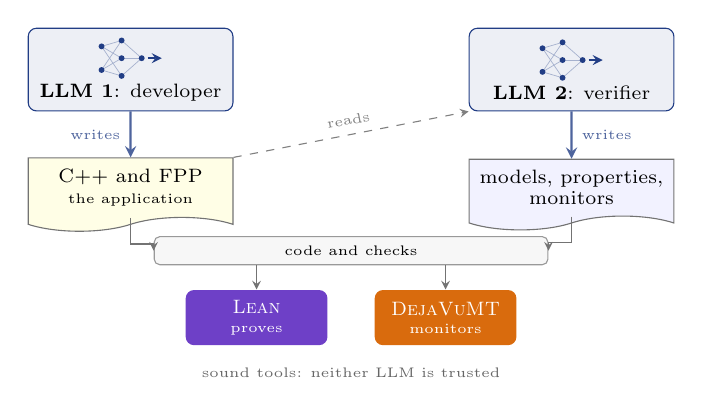
\begin{tikzpicture}[
  font=\scriptsize, >=stealth,
  llm/.style={draw=iconcol, fill=iconcol!8, rounded corners=3pt, align=center,
              minimum width=2.6cm, minimum height=1.05cm},
  art/.style={doc, fill=yellow!10},
  chk/.style={doc, fill=blue!5},
  doc/.style={draw=black!55, align=center, minimum width=2.6cm, minimum height=0.8cm,
              tape, tape bend top=none, tape bend height=5pt, inner ysep=4pt},
  tool/.style={rounded corners=3pt, align=center, text=white, font=\scriptsize\bfseries,
               minimum width=1.8cm, minimum height=0.7cm}
]
  % the developer side
  \node[llm] (dev) at (0, 1.25) {\iconllm[0.75]\\[1pt]{\bf LLM 1}: developer};
  \node[art] (code) at (0, -0.25) {C++ and FPP\\{\tiny the application}};
  \draw[->, thick, iconcol!80] (dev) -- node[left, font=\tiny] {writes} (code);

  % the verifier side
  \node[llm] (ver) at (5.6, 1.25) {\iconllm[0.75]\\[1pt]{\bf LLM 2}: verifier};
  \node[chk] (spec) at (5.6, -0.25) {models, properties,\\monitors};
  \draw[->, thick, iconcol!80] (ver) -- node[right, font=\tiny] {writes} (spec);
  \draw[->, dashed, black!50] (code.north east) -- node[above, sloped, font=\tiny] {reads} (ver.south west);

  \pause

  % the judges: both read the code and the checks
  \node[tool, fill=leancol] (lean) at (1.6, -1.9) {\lean{}\\[-1pt]{\tiny\mdseries proves}};
  \node[tool, fill=dejavucol] (dvm) at (4.0, -1.9) {\dejavumt{}\\[-1pt]{\tiny\mdseries monitors}};
  \node[draw=black!40, fill=black!3, rounded corners=2pt, minimum width=5.0cm,
        minimum height=0.32cm, font=\tiny] (both) at (2.8, -1.05) {code and checks};
  \draw[->, black!55] (code.south) -- ++(0,-0.33) -| (both.west);
  \draw[->, black!55] (spec.south) -- ++(0,-0.33) -| (both.east);
  \draw[->, black!55] (both.south -| lean.north) -- (lean.north);
  \draw[->, black!55] (both.south -| dvm.north) -- (dvm.north);
  \node[font=\tiny, text=black!60] at (2.8, -2.6) {sound tools: neither LLM is trusted};
\end{tikzpicture}\par}

\pause
\vspace{0.2cm}

{\centering\small The {\bf disagreements} are the findings.\par}

\end{frame}
%----------------------------------------
\begin{frame}
  \frametitle{\fcheck{}: the proof and monitor pipelines} \small

\vspace{-0.2cm}

{\centering
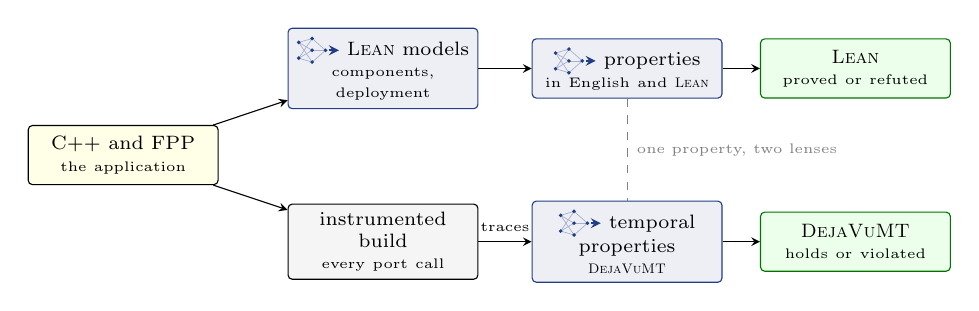
\begin{tikzpicture}[
  font=\scriptsize, >=stealth,
  b/.style={draw, rounded corners=1.5pt, align=center, inner sep=3pt,
            minimum height=0.75cm, text width=2.2cm},
  llm/.style={b, fill=iconcol!8, draw=iconcol},
  sound/.style={b, fill=green!8, draw=green!45!black}
]
  \node[b, fill=yellow!10] (src) at (0,0) {C++ and FPP\\{\tiny the application}};

  \node[llm]   (model) at (3.3, 1.1)  {\iconllm[0.5]\ \lean{} models\\{\tiny components, deployment}};
  \node[llm]   (props) at (6.4, 1.1)  {\iconllm[0.5]\ properties\\{\tiny in English and \lean{}}};
  \node[sound] (prove) at (9.3, 1.1)  {\lean{}\\{\tiny proved or refuted}};

  \node[b, fill=black!4] (inst) at (3.3,-1.1) {instrumented build\\{\tiny every port call}};
  \node[llm]   (spec) at (6.4,-1.1) {\iconllm[0.5]\ temporal properties\\{\tiny \dejavumt{}}};
  \node[sound] (mon)  at (9.3,-1.1) {\dejavumt{}\\{\tiny holds or violated}};

  \draw[->] (src) -- (model);  \draw[->] (model) -- (props); \draw[->] (props) -- (prove);
  \draw[->] (src) -- (inst);   \draw[->] (inst) -- node[above, font=\tiny] {traces} (spec);
  \draw[->] (spec) -- (mon);
  \draw[dashed, gray] (props) -- node[right, font=\tiny, gray] {one property, two lenses} (spec);
\end{tikzpicture}\par}

\vspace{0.3cm}

\begin{itemize}\small
\item \lean{}: a theorem prover; proofs are checked by its small kernel.
\item \dejavumt{} (work with Doron Peled): first-order past and future time logic with
      time bounds ({\tt P[<=10]}, {\tt F[<=1000]}), checked over a trace with an SMT solver.
\item Works on {\bf any} \fprime{} application: reads the FPP, topology and dictionary.
\end{itemize}

\end{frame}
        %  3 min   the setting, the idea, the tool
%----------------------------------------
\begin{frame}
  \frametitle{The Deployment page} \small

\vspace{-0.15cm}
{\centering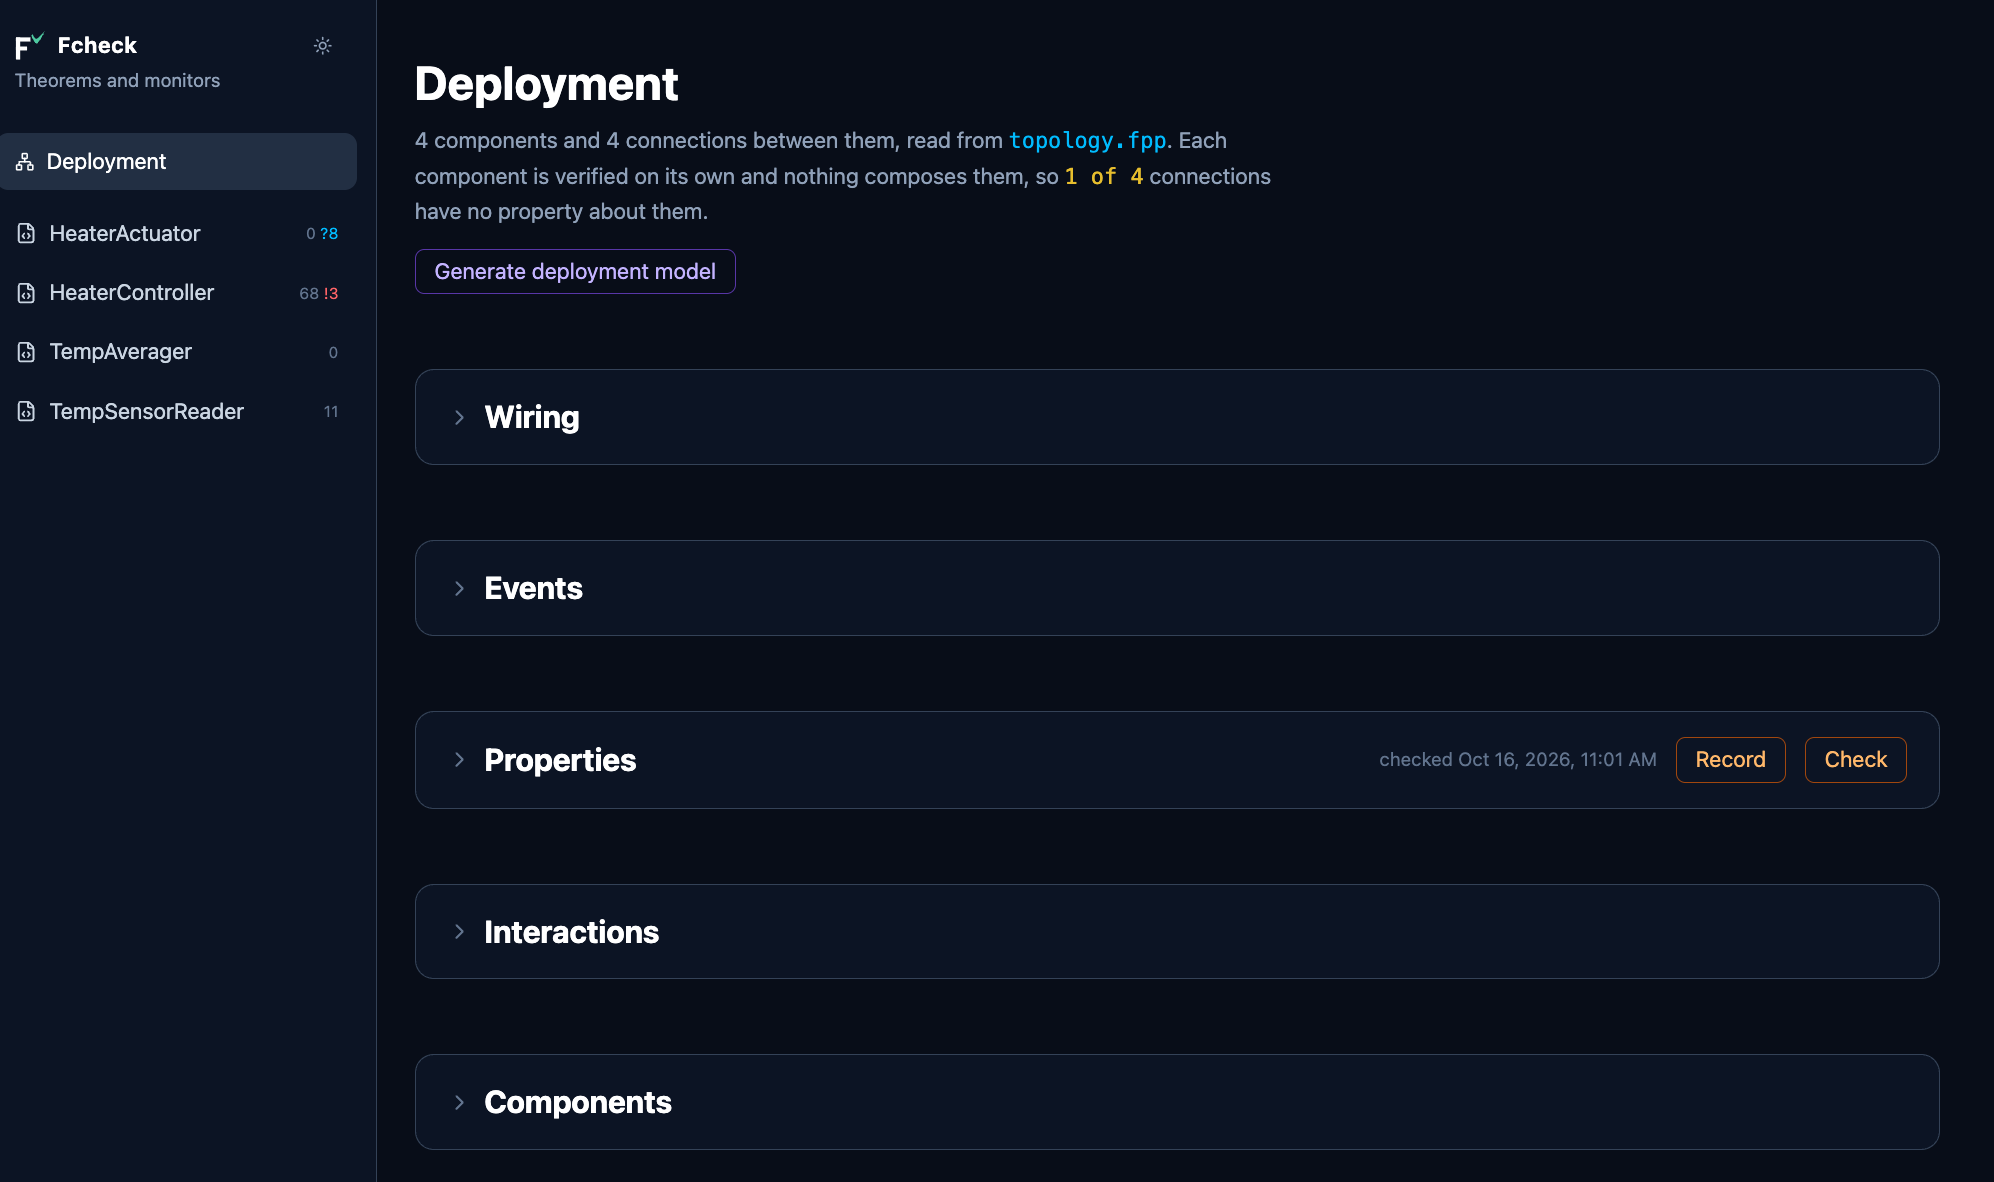
\includegraphics[width=\textwidth,height=0.74\textheight,keepaspectratio]{figures/1-deployment.png}\par}

\vspace{0.1cm}
{\scriptsize Generated from {\tt topology.fpp}}

\end{frame}

%----------------------------------------
\begin{frame}
  \frametitle{The wiring} \small

\vspace{-0.15cm}
{\centering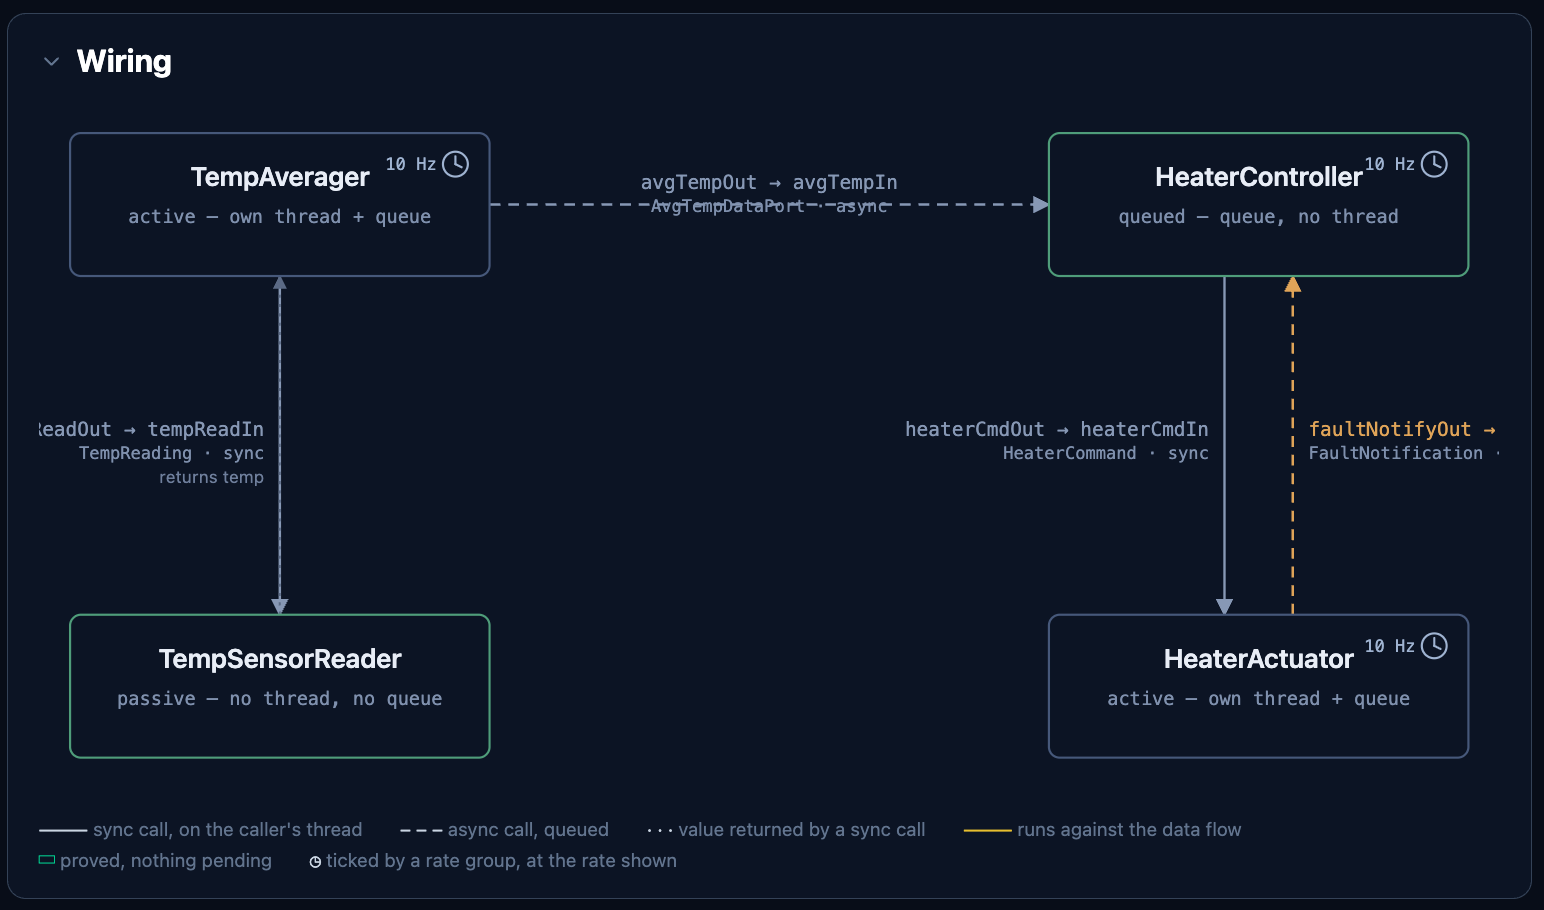
\includegraphics[width=\textwidth,height=0.74\textheight,keepaspectratio]{figures/2-wiring.png}\par}

\vspace{0.1cm}
{\scriptsize Read from the topology: sync and async ports, rate groups, data flow.}

\end{frame}

%----------------------------------------
\begin{frame}
  \frametitle{What temporal properties can talk about} \small

\vspace{-0.15cm}
{\centering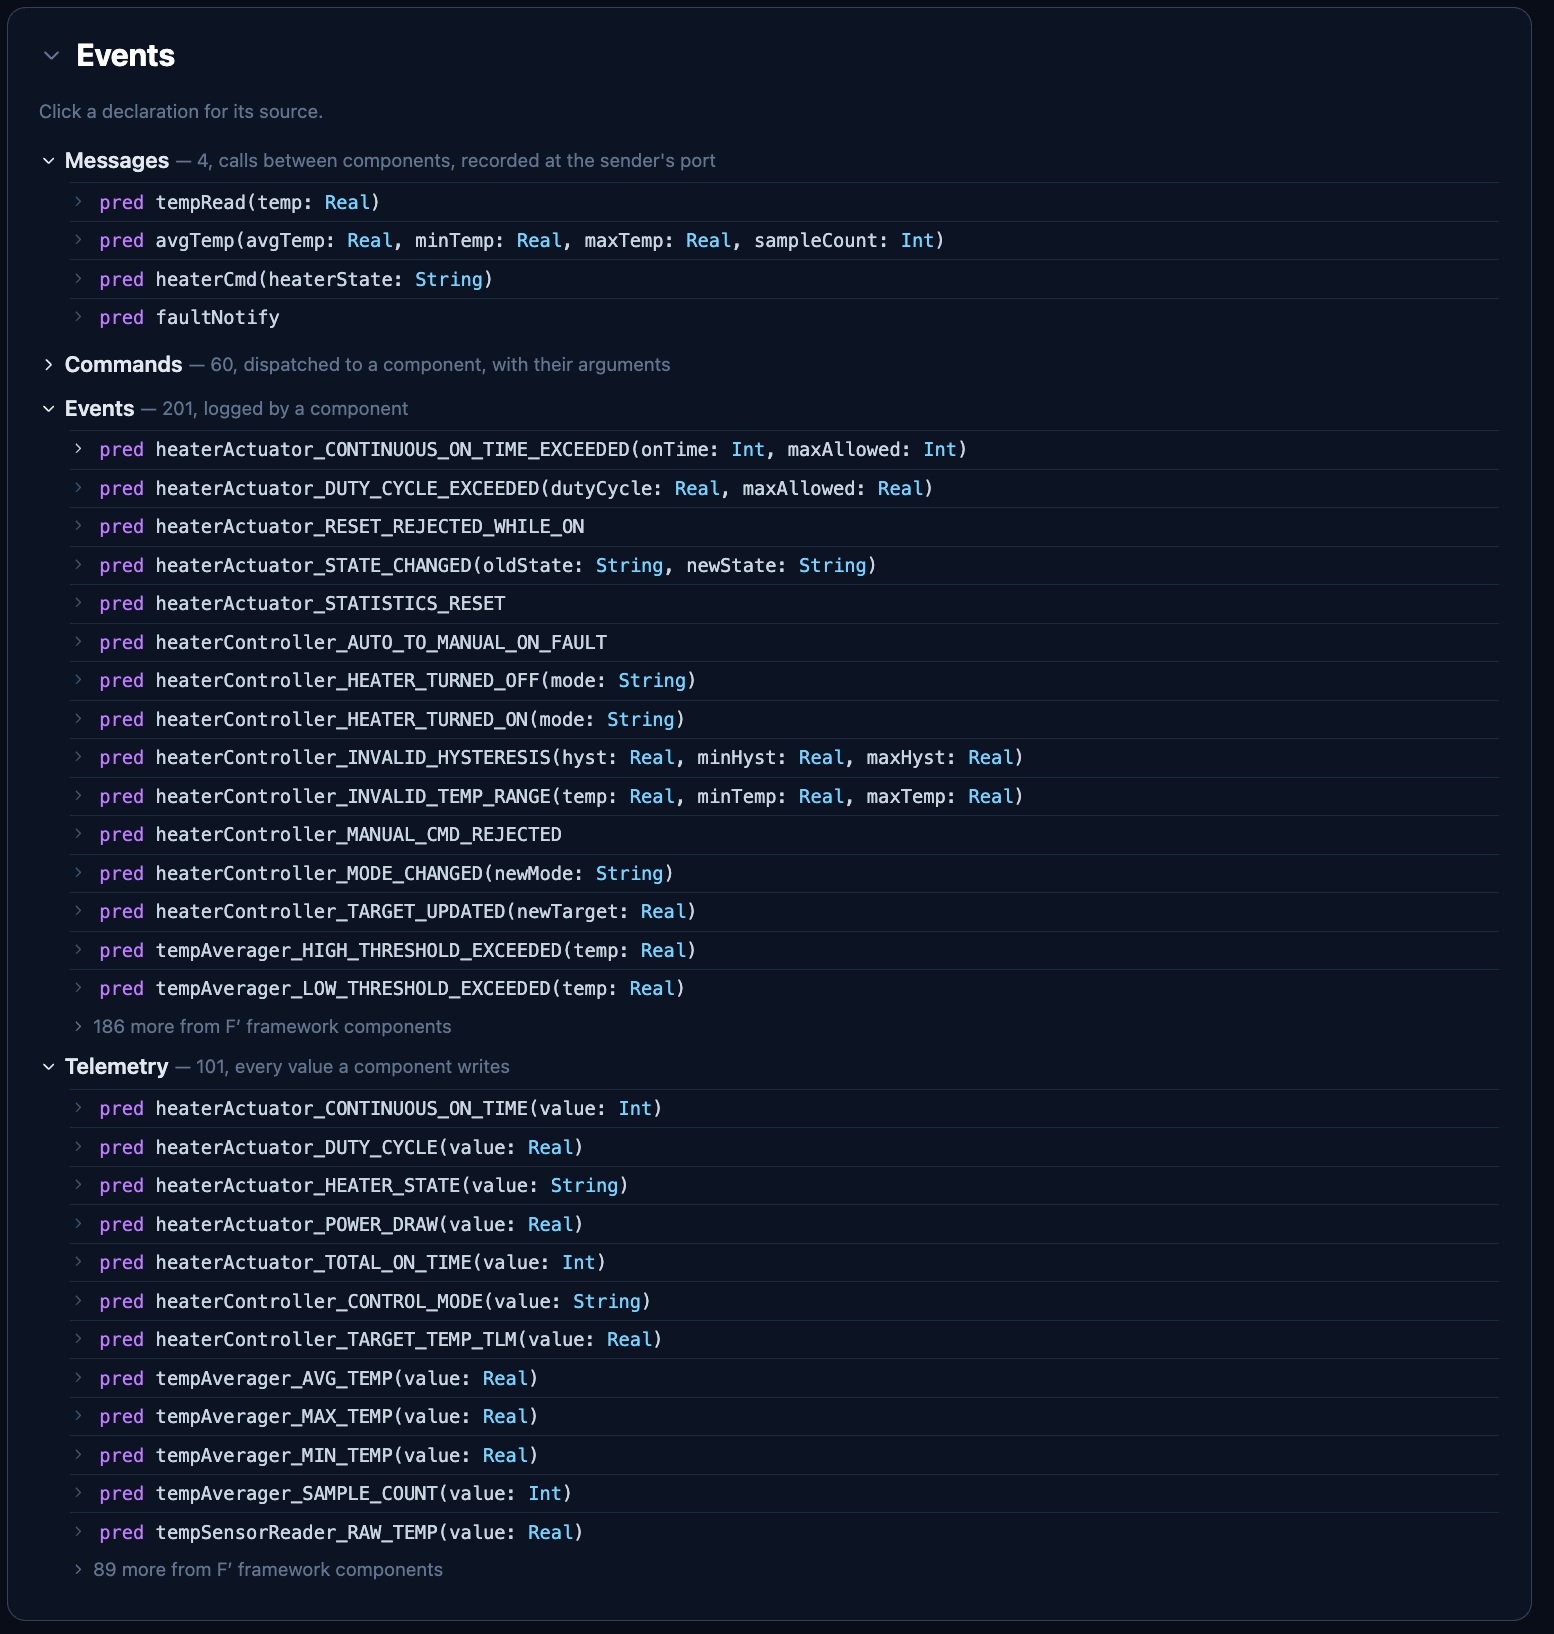
\includegraphics[width=\textwidth,height=0.74\textheight,keepaspectratio]{figures/3-events.png}\par}

\vspace{0.1cm}
{\scriptsize Generated from the \fprime{} dictionary: every message, command, event and telemetry channel, typed.}

\end{frame}

%----------------------------------------
\begin{frame}
  \frametitle{Deployment properties: \dejavumt{}} \small

\vspace{-0.15cm}
{\centering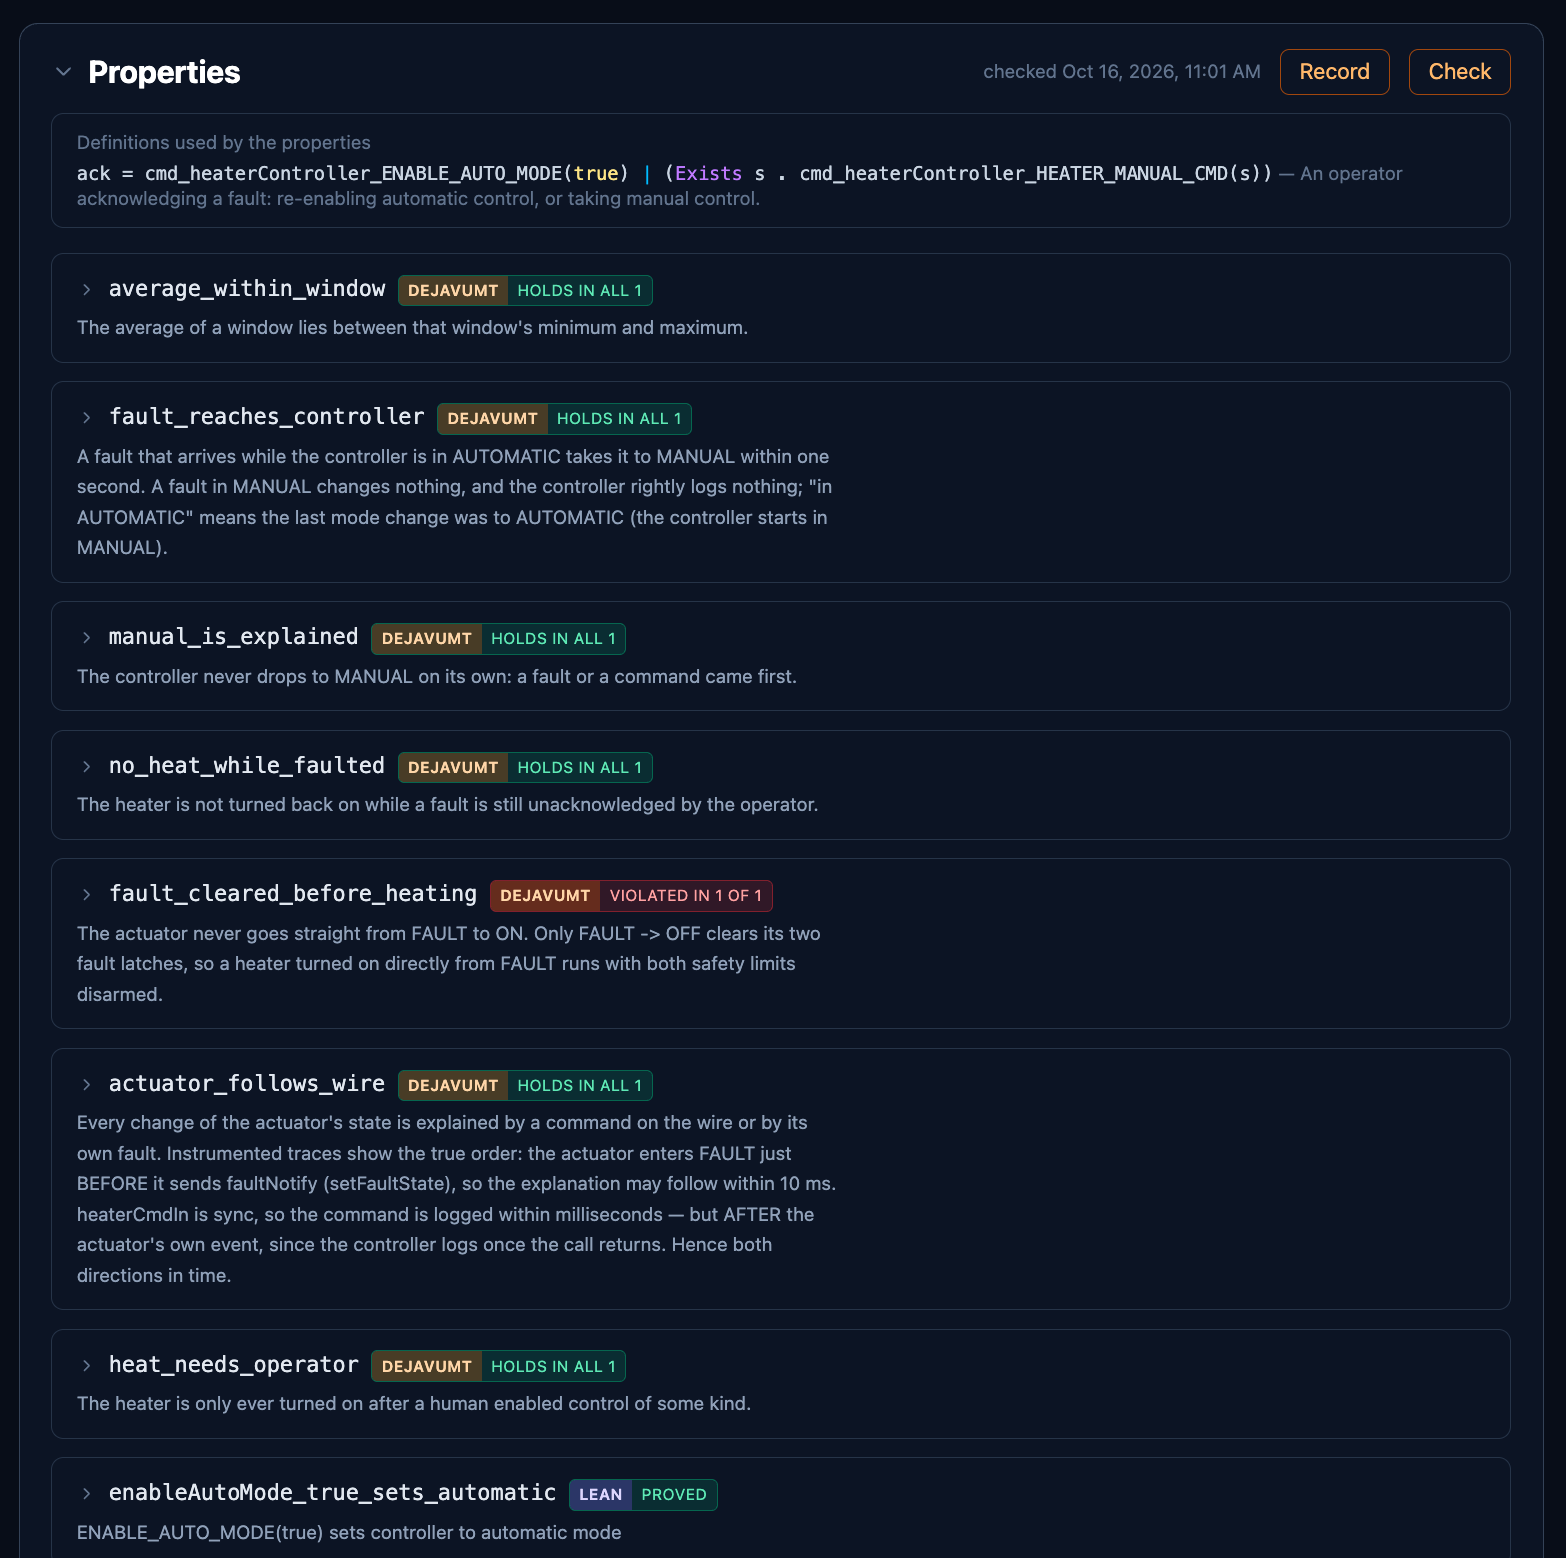
\includegraphics[width=\textwidth,height=0.74\textheight,keepaspectratio]{figures/4-properties1.png}\par}

\vspace{0.1cm}
{\scriptsize Checked on recorded runs of the instrumented system. One is violated.}

\end{frame}

%----------------------------------------
\begin{frame}
  \frametitle{Deployment properties: \lean{}} \small

\vspace{-0.15cm}
{\centering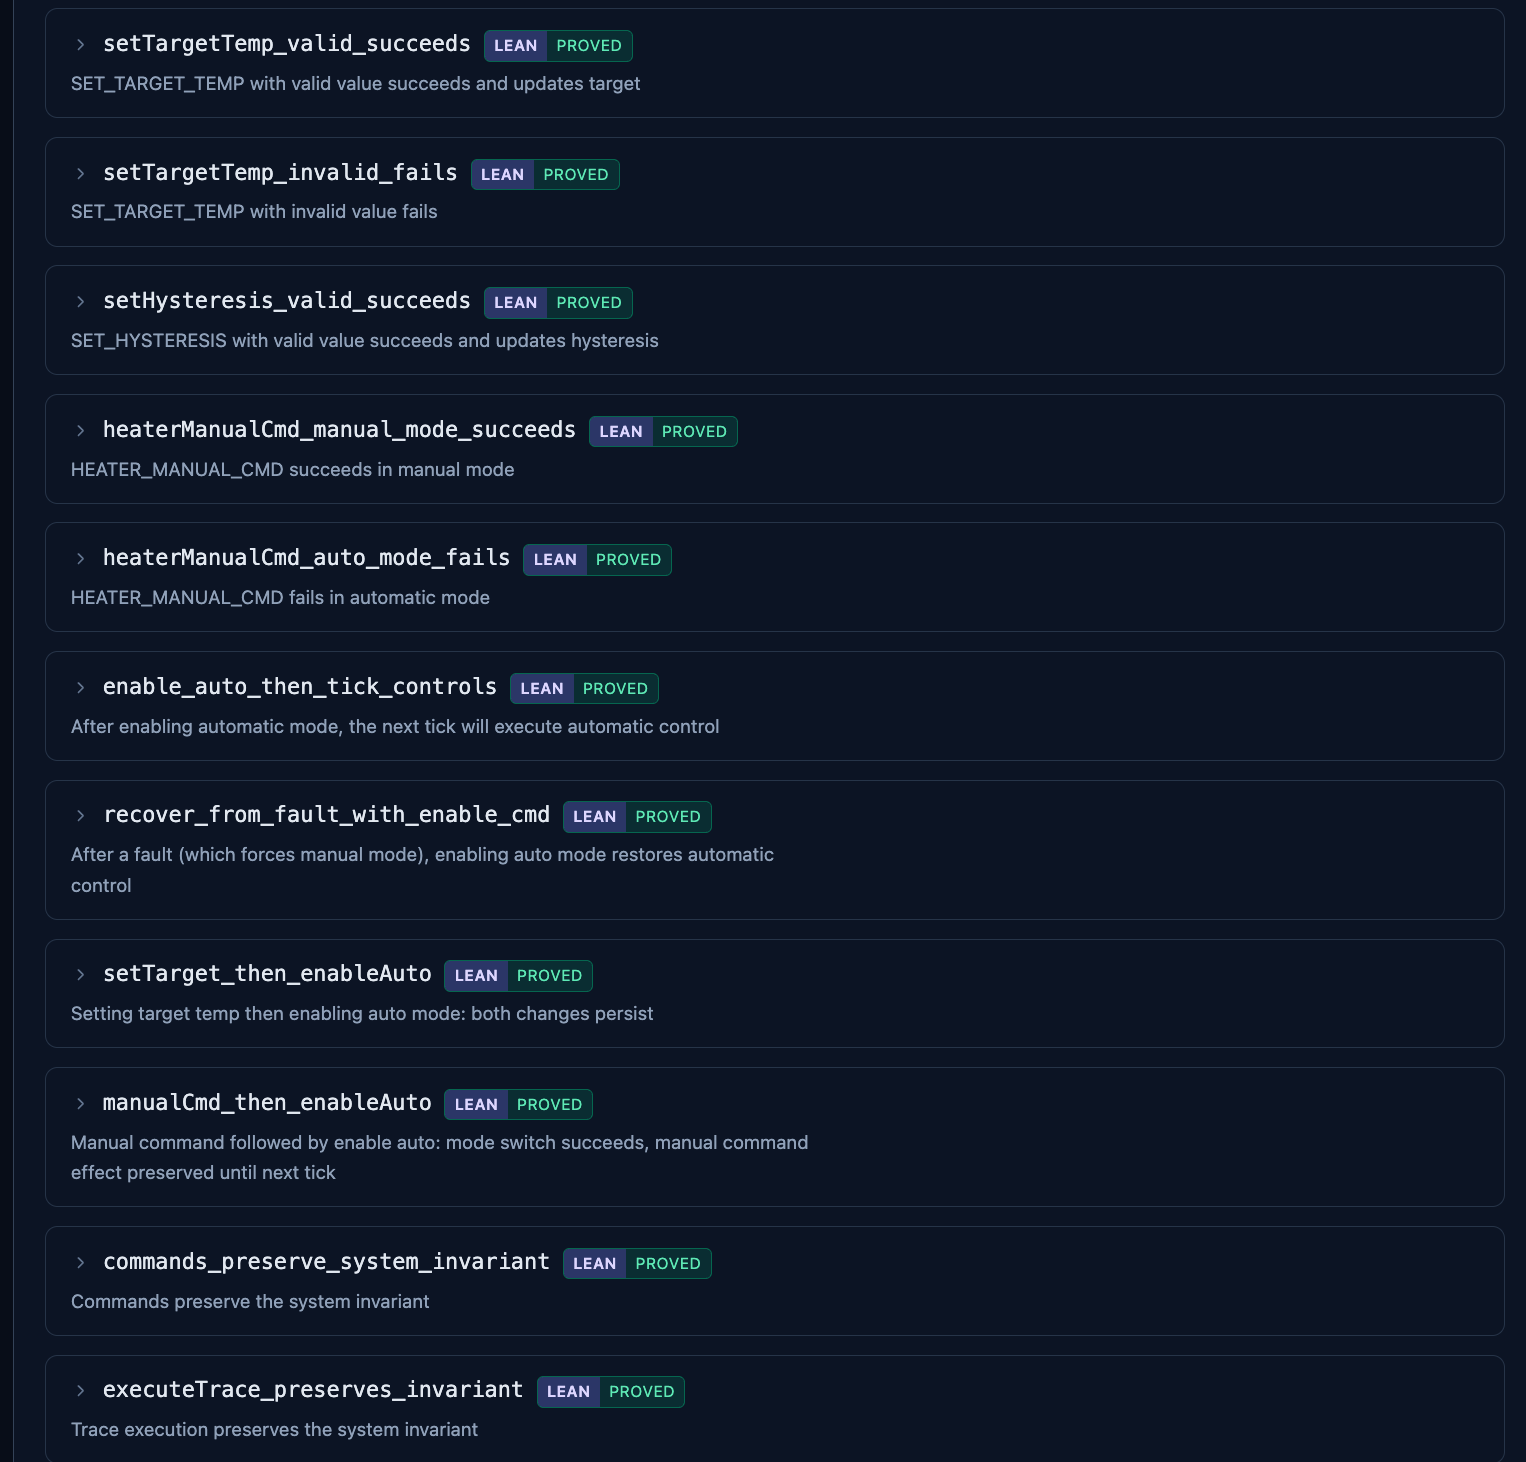
\includegraphics[width=\textwidth,height=0.74\textheight,keepaspectratio]{figures/5-properties2.png}\par}

\vspace{0.1cm}
{\scriptsize Theorems over the system model.}

\end{frame}

%----------------------------------------
\begin{frame}
  \frametitle{A component page} \small

\vspace{-0.15cm}
{\centering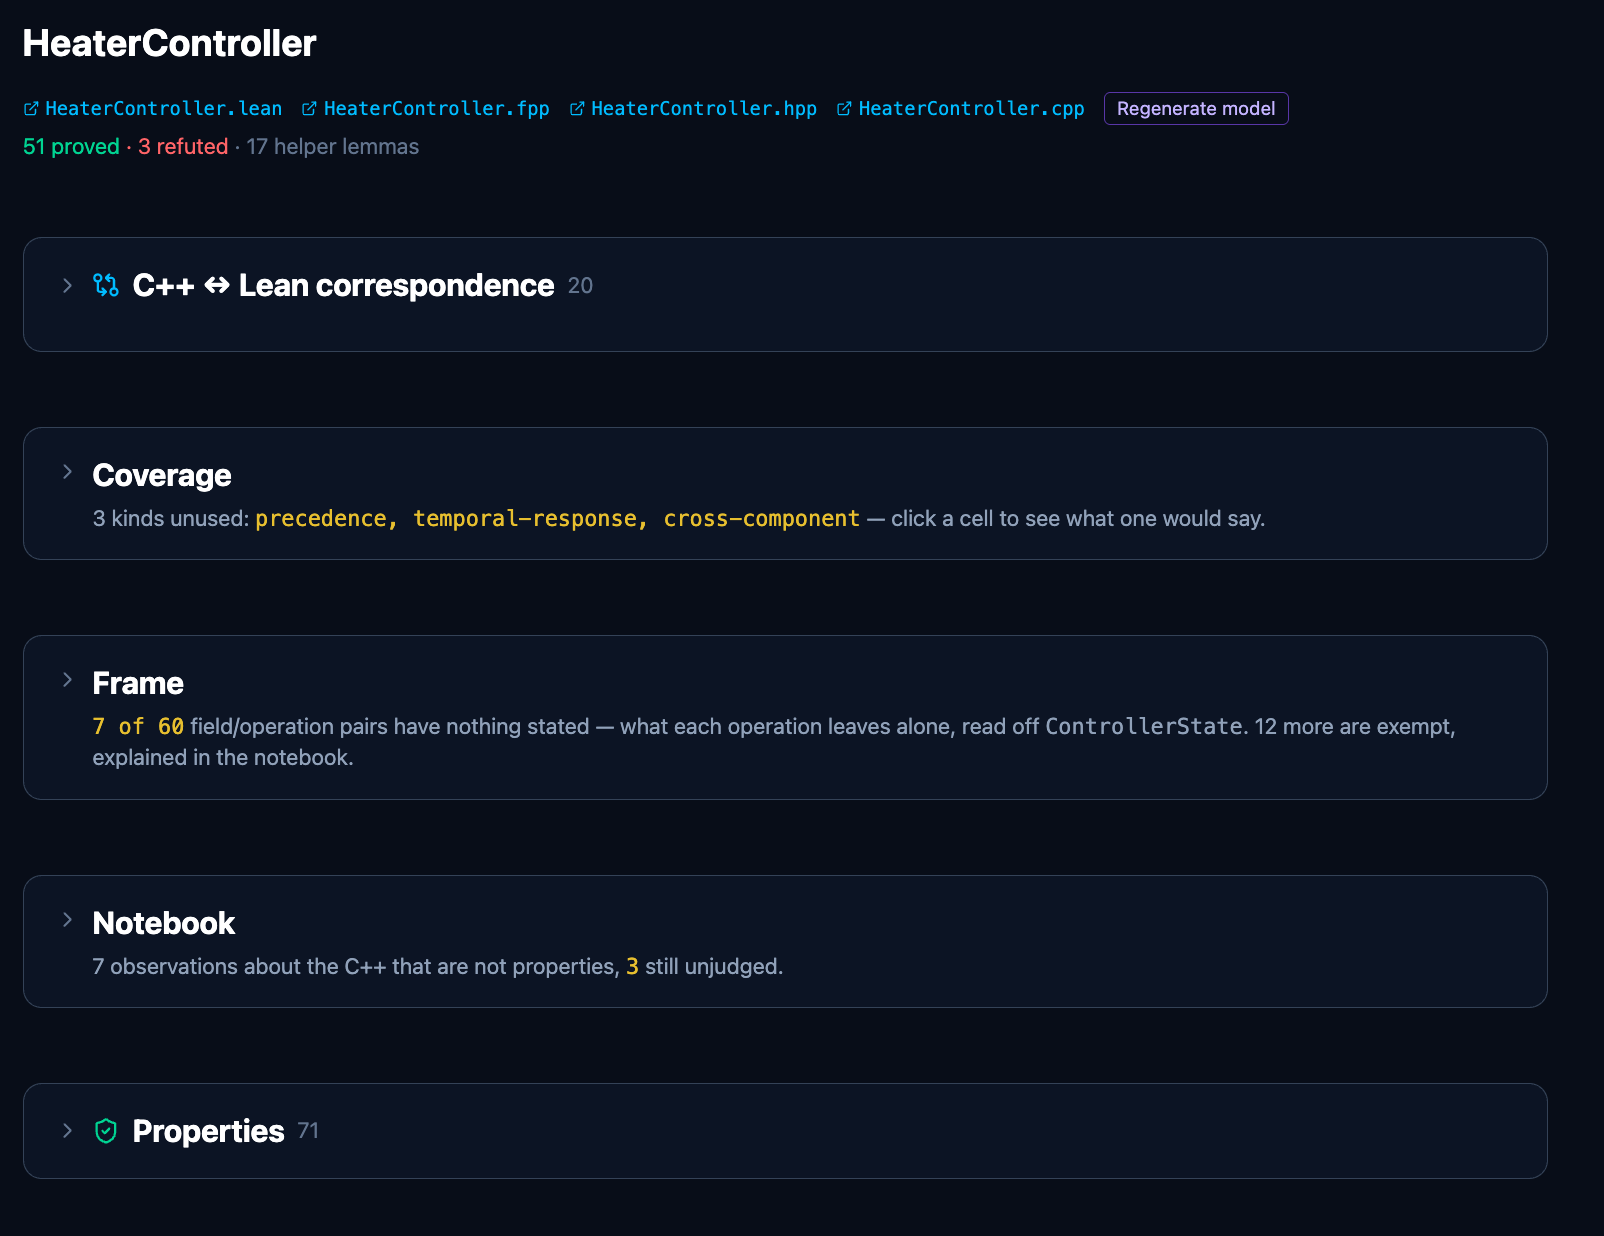
\includegraphics[width=\textwidth,height=0.74\textheight,keepaspectratio]{figures/6-heatercontroller.png}\par}

\end{frame}

%----------------------------------------
\begin{frame}
  \frametitle{The C++ $\leftrightarrow$ \lean{} correspondence} \small

\vspace{-0.15cm}
{\centering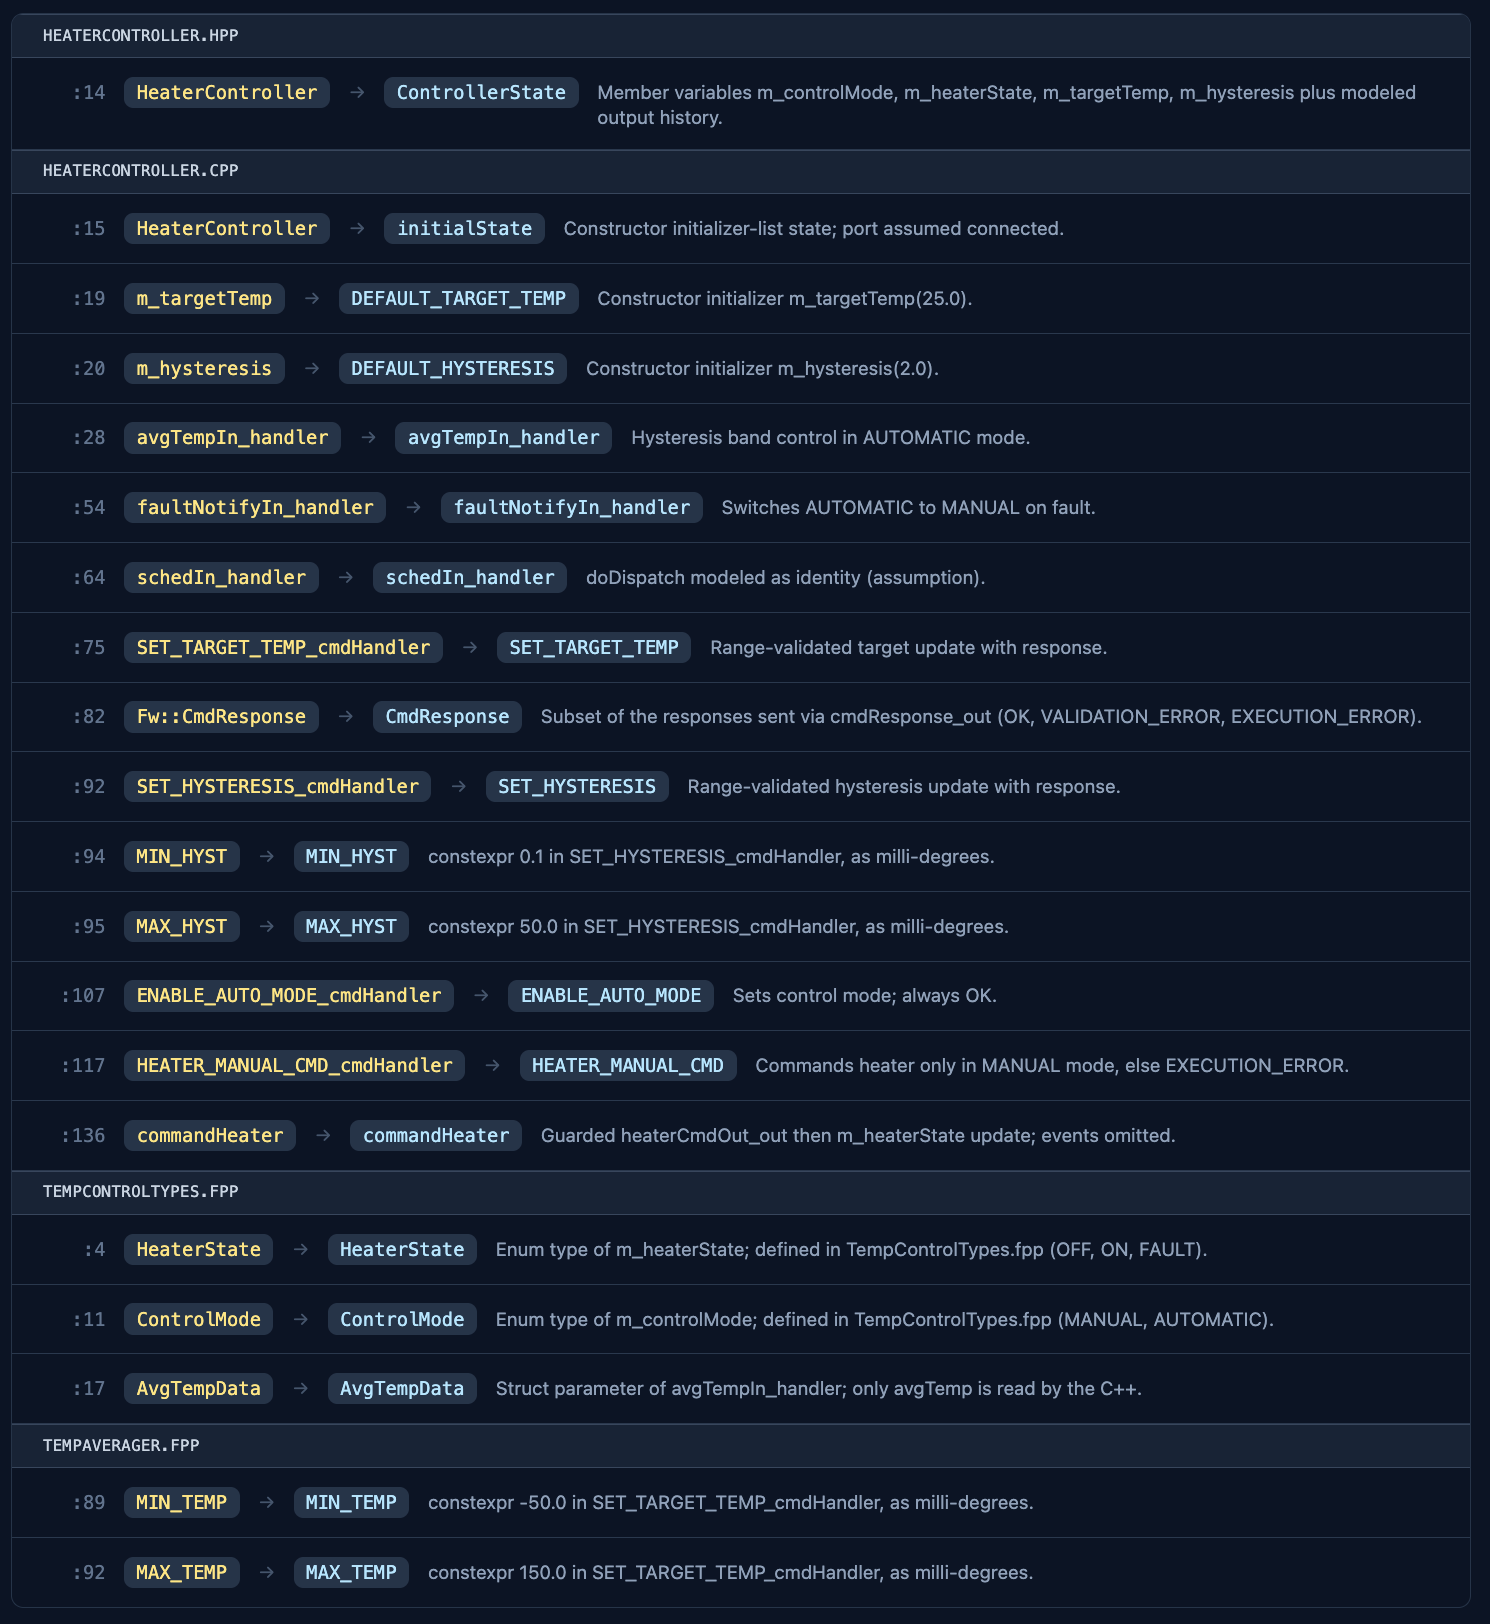
\includegraphics[width=\textwidth,height=0.74\textheight,keepaspectratio]{figures/7-cpp-lean.png}\par}

\vspace{0.1cm}
{\scriptsize What each C++ element became in the model.}

\end{frame}

%----------------------------------------
\begin{frame}
  \frametitle{Clicking a row opens both sides} \small

\vspace{-0.15cm}
{\centering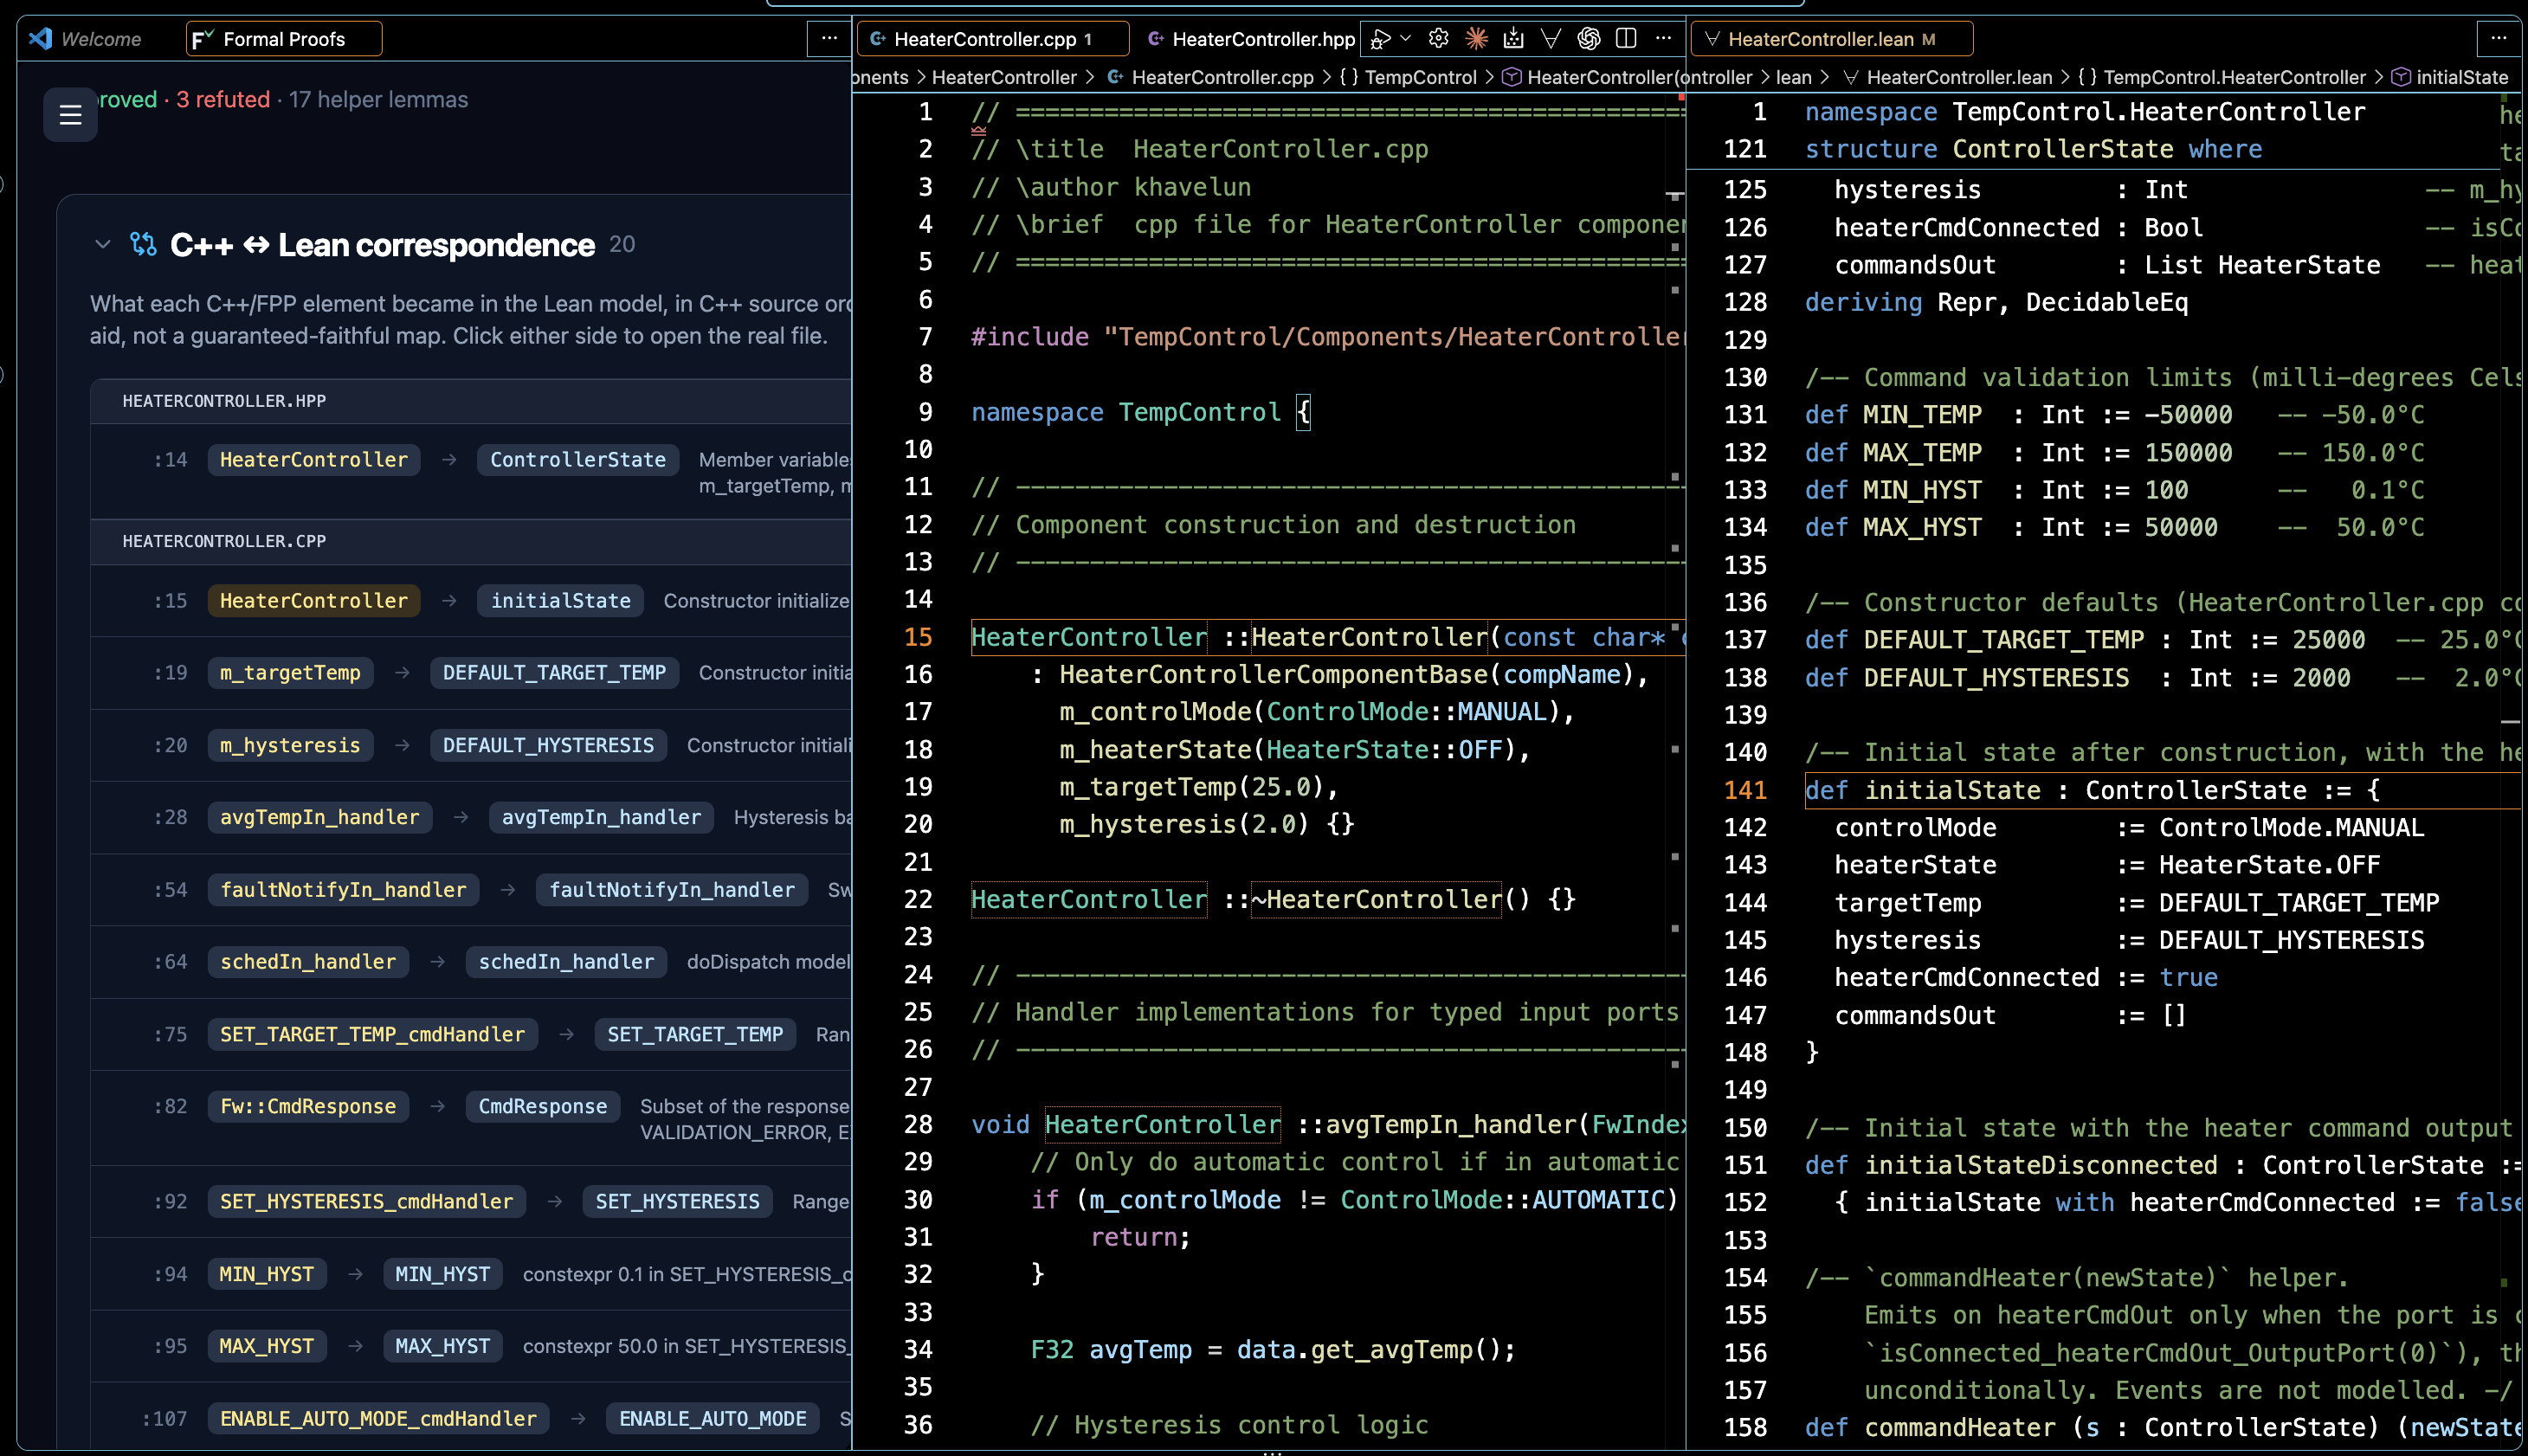
\includegraphics[width=\textwidth,height=0.74\textheight,keepaspectratio]{figures/8-init-state.png}\par}

\vspace{0.1cm}
{\scriptsize The C++ constructor and the \lean{} {\tt initialState}, side by side.}

\end{frame}

%----------------------------------------
\begin{frame}
  \frametitle{The handler and its model} \small

\vspace{-0.15cm}
{\centering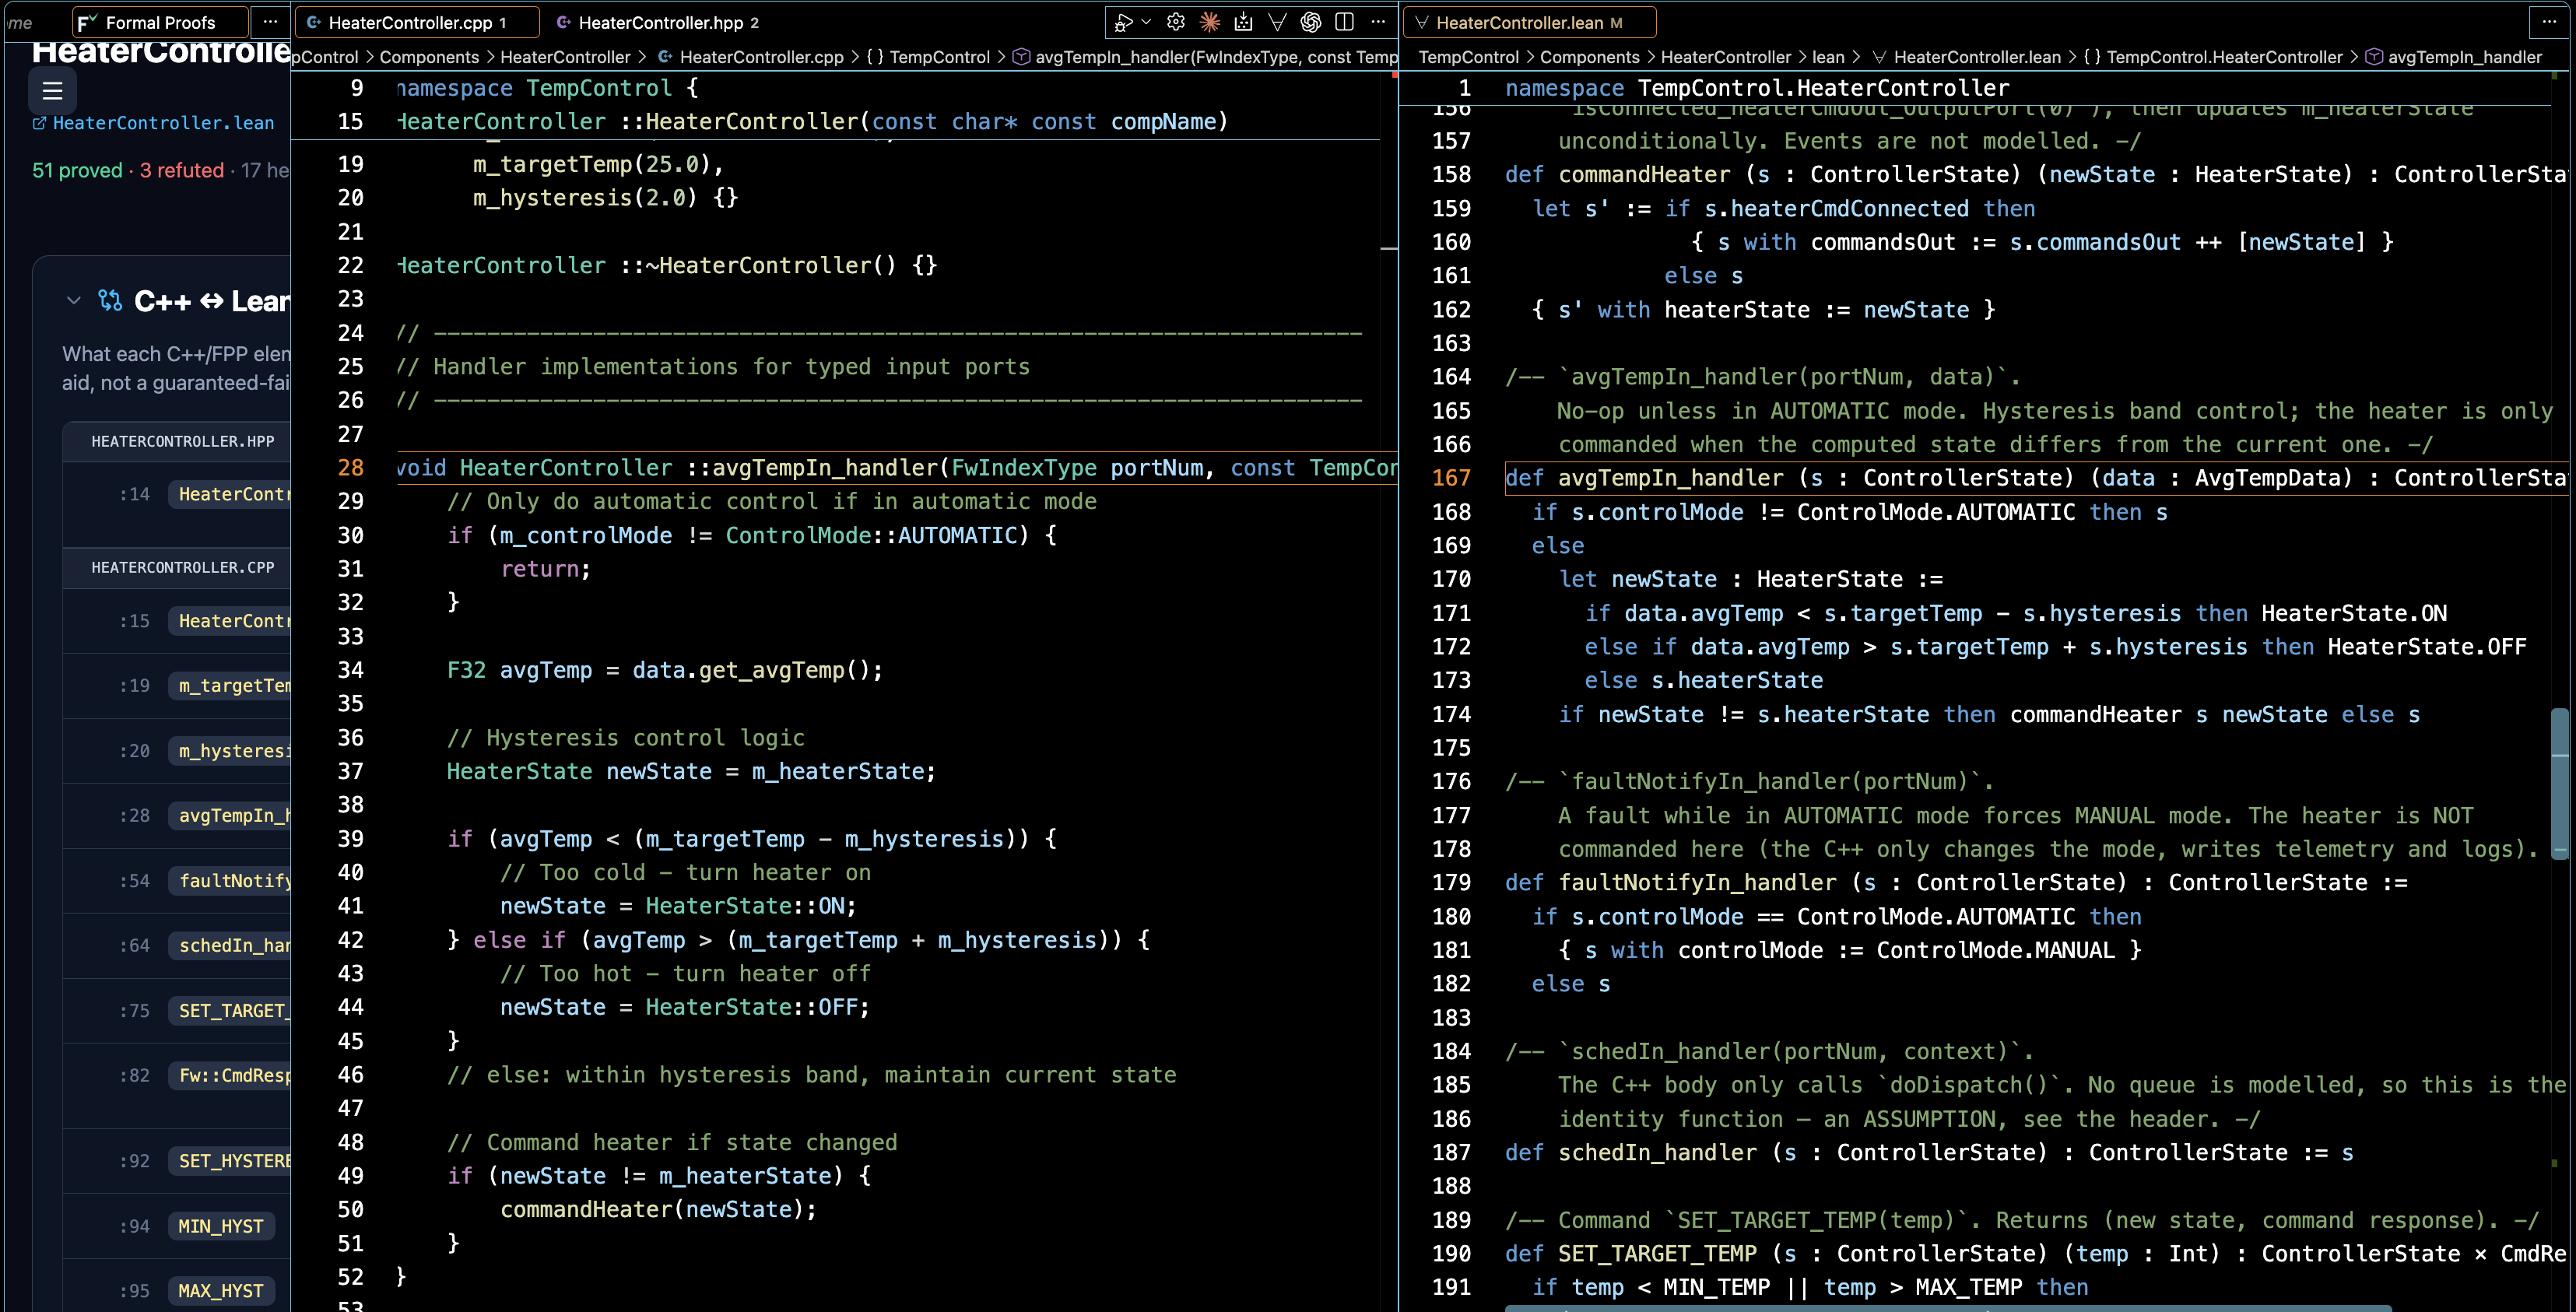
\includegraphics[width=\textwidth,height=0.74\textheight,keepaspectratio]{figures/9-handler.png}\par}

\vspace{0.1cm}
{\scriptsize {\tt avgTempIn\_handler} in C++ and in \lean{}: the model tracks the code line for line.}

\end{frame}

%----------------------------------------
\begin{frame}
  \frametitle{Properties, grouped by C++ entry point} \small

\vspace{-0.15cm}
{\centering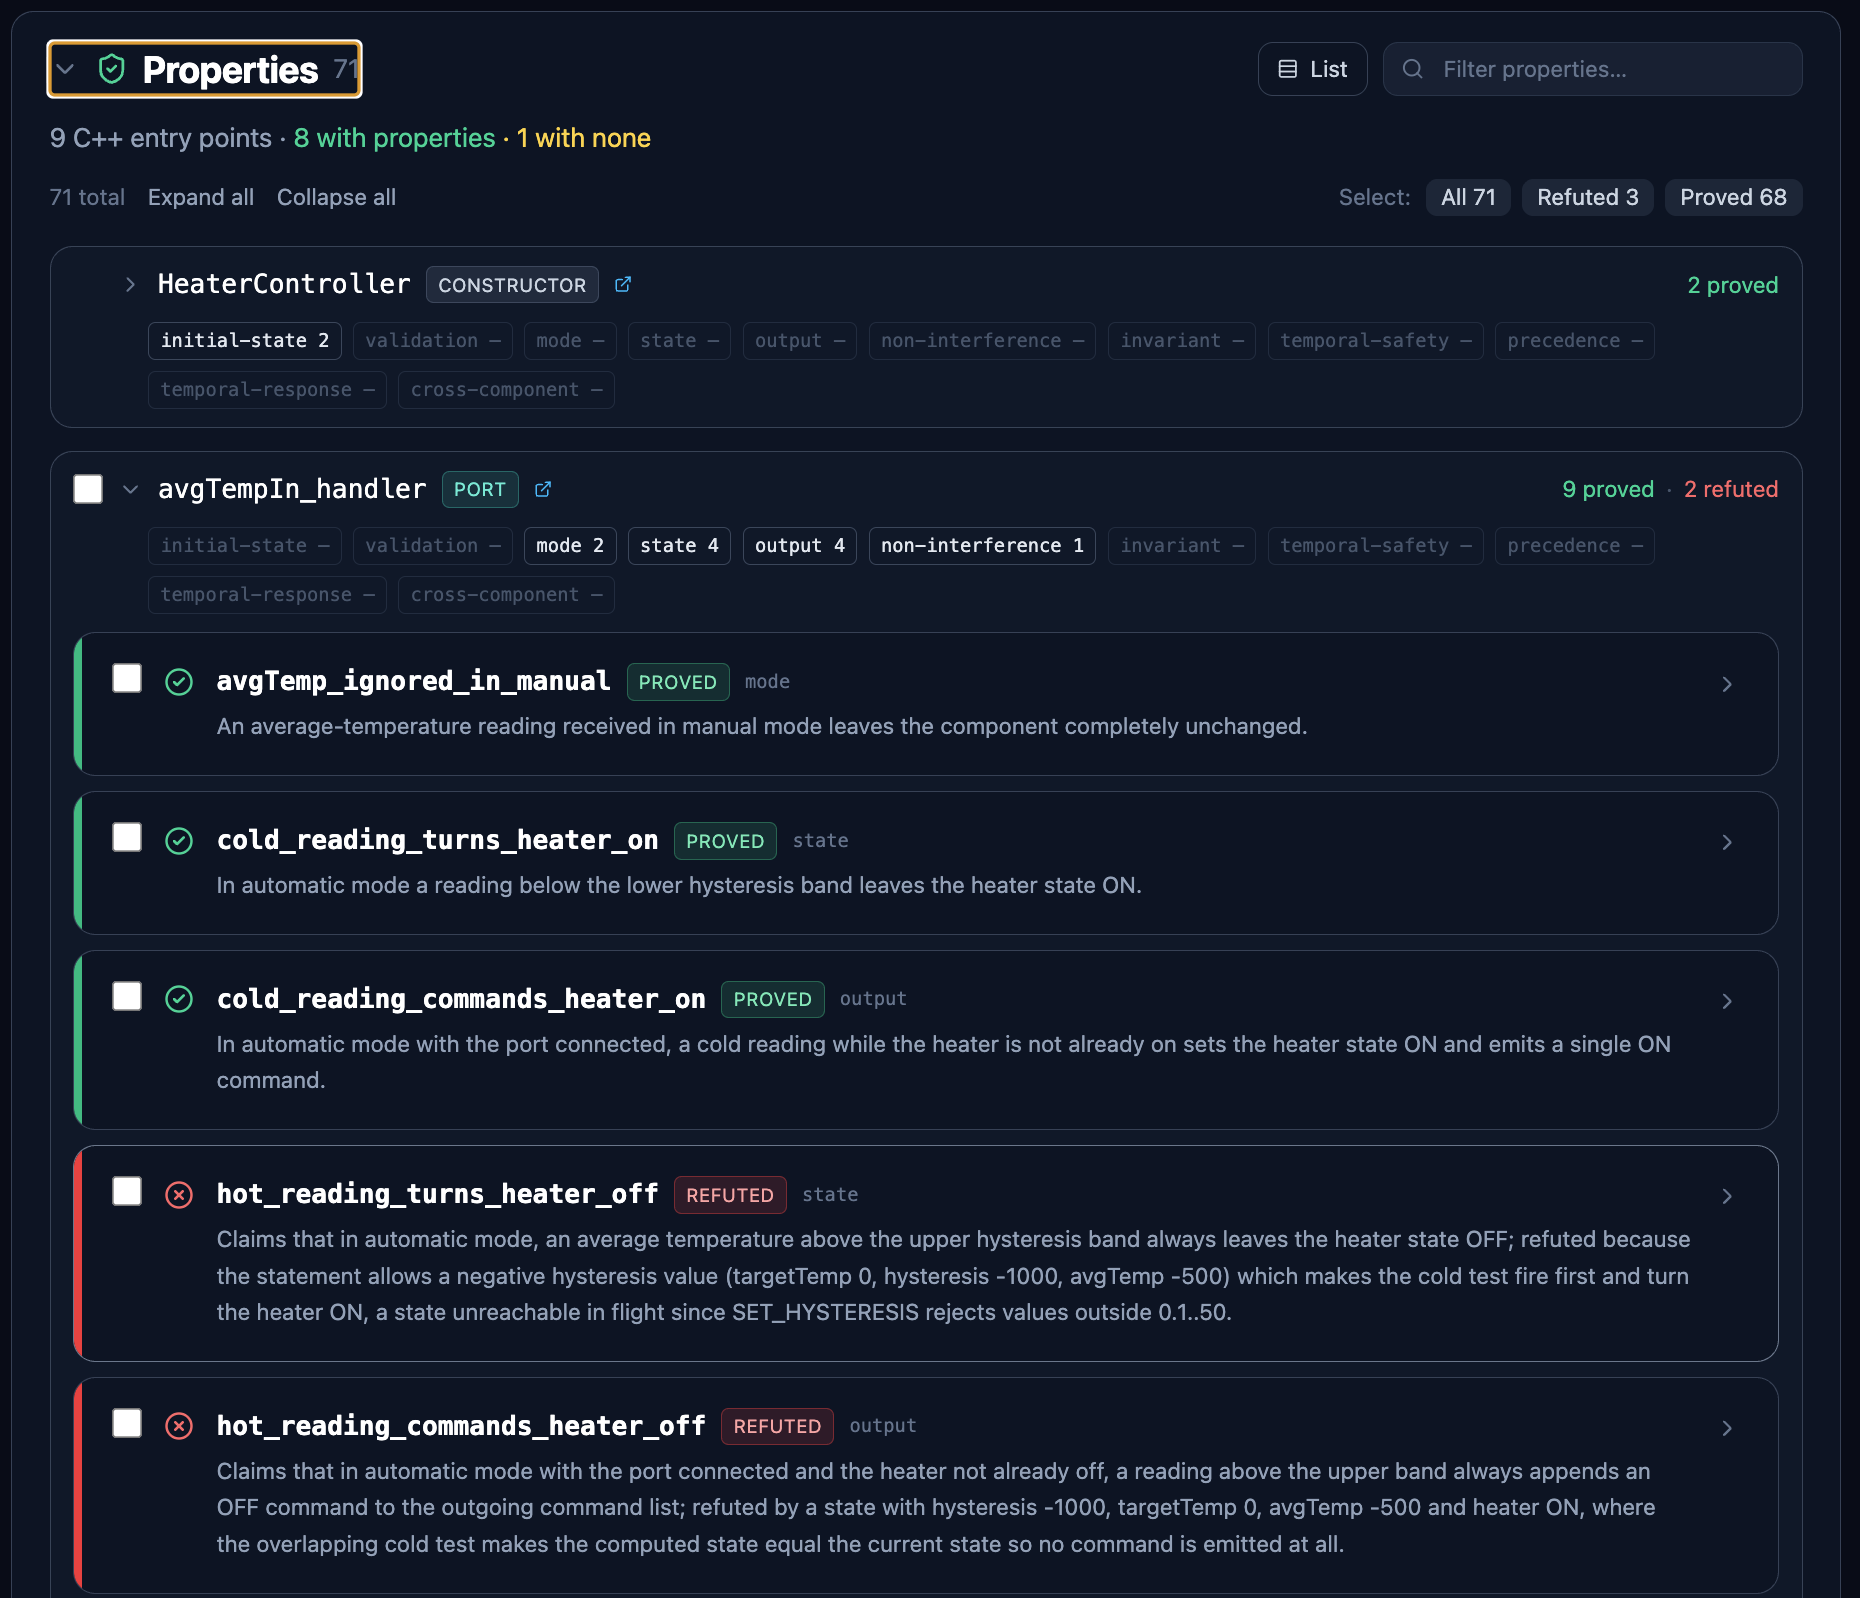
\includegraphics[width=\textwidth,height=0.74\textheight,keepaspectratio]{figures/10-properties.png}\par}

\vspace{0.1cm}
{\scriptsize Each with its English, its kind and its status. Two of these are refuted.}

\end{frame}

%----------------------------------------
\begin{frame}
  \frametitle{A refuted property, expanded} \small

\vspace{-0.15cm}
{\centering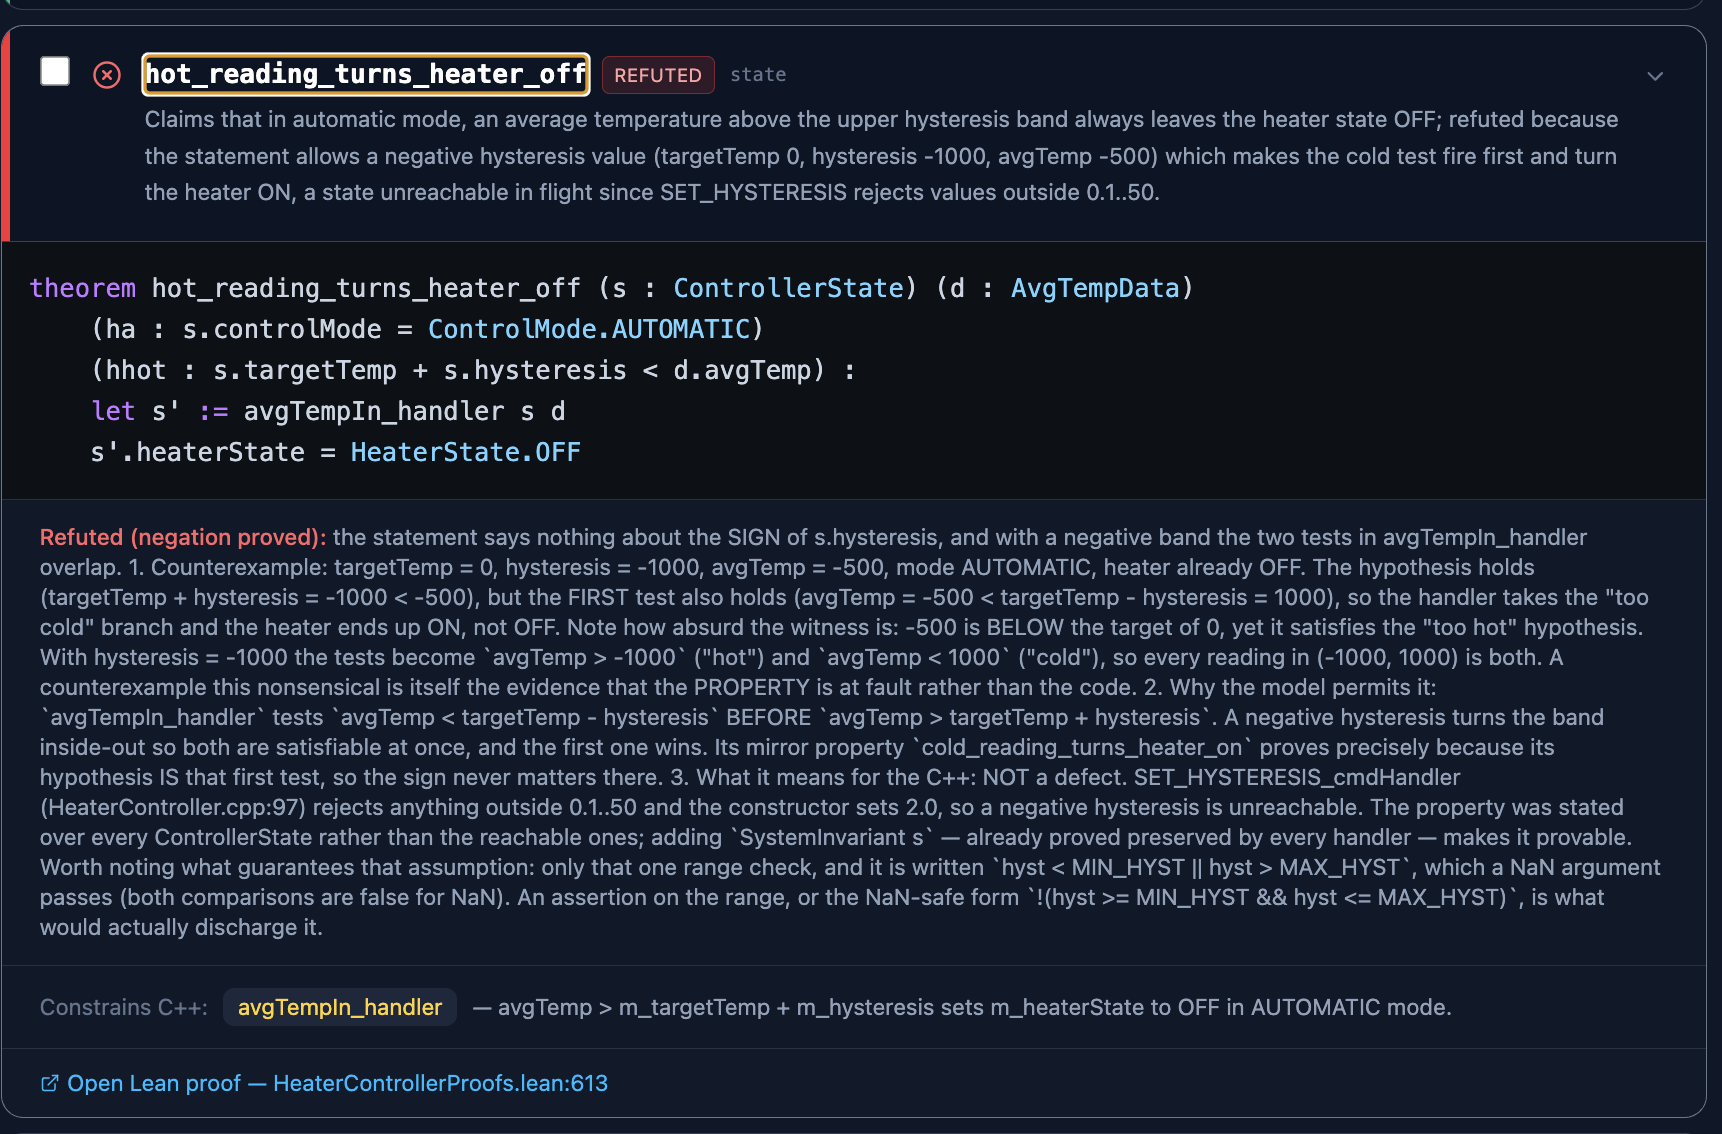
\includegraphics[width=\textwidth,height=0.73\textheight,keepaspectratio]{figures/11-lean-heater-off.png}\par}

\vspace{0.1cm}
{\scriptsize The statement, the counterexample, why the model allows it, and what it means
for the C++.}

\end{frame}
         %  5 min   the tool, in screenshots
%----------------------------------------
\begin{frame}[fragile]
  \frametitle{Recall: the heater controller's hysteresis} \small
\leanbadge{1}{refuted}{red!75!black}

\vspace{-0.35cm}
\whereami{ctl}

\vspace{-0.1cm}
In automatic mode, every average reading goes through two tests:

\begin{lstlisting}[style=cpp]
if      (avgTemp < (m_targetTemp - m_hysteresis)) newState = ON;   // too cold
else if (avgTemp > (m_targetTemp + m_hysteresis)) newState = OFF;  // too hot
if (newState != m_heaterState) commandHeater(newState);
\end{lstlisting}

\pause
\vspace{0.2cm}

With the defaults, target 25\,$^\circ$C and hysteresis {\bf +2}\,$^\circ$C:

\vspace{0.15cm}
{\centering
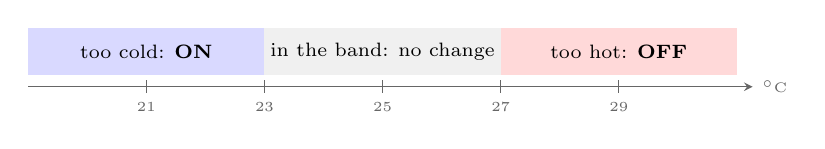
\begin{tikzpicture}[font=\scriptsize, >=stealth]
  \draw[->, black!60] (0,0) -- (9.2,0) node[right, font=\tiny] {$^\circ$C};
  \foreach \x/\t in {1.5/21, 3/23, 4.5/25, 6/27, 7.5/29} {
    \draw[black!60] (\x,0.08) -- (\x,-0.08) node[below, font=\tiny] {\t};
  }
  \fill[blue!15] (0,0.15) rectangle (3,0.75);
  \node at (1.5,0.45) {too cold: {\bf ON}};
  \fill[black!6] (3,0.15) rectangle (6,0.75);
  \node at (4.5,0.45) {in the band: no change};
  \fill[red!15] (6,0.15) rectangle (9,0.75);
  \node at (7.5,0.45) {too hot: {\bf OFF}};
\end{tikzpicture}\par}

\end{frame}
%----------------------------------------
\begin{frame}[fragile]
  \frametitle{A proof attempt that failed --- usefully} \small
\leanbadge{1}{refuted}{red!75!black}

Proposed: {\em ``a hot reading turns the heater off''}.

\begin{lstlisting}[language=lean4]
theorem hot_reading_commands_heater_off (s : ControllerState) (d : AvgTempData)
    (ha : s.controlMode = ControlMode.AUTOMATIC)
    (hc : s.heaterCmdConnected = true)
    (hon : s.heaterState $\neq$ HeaterState.OFF)
    (hhot : s.targetTemp + s.hysteresis < d.avgTemp) :
    let s' := avgTempIn_handler s d
    s'.commandsOut = s.commandsOut ++ [HeaterState.OFF]
\end{lstlisting}

\vspace{-0.15cm}
\pause

{\bf Refuted}, with a counterexample: target 25\,$^\circ$C, hysteresis $-2\,^\circ$C,
heater ON, reading 26\,$^\circ$C.

\begin{itemize}\small
\item 26\,$^\circ$C is hot. But $26 < 25 - (-2)$: it
      also counts as ``too cold'', that test comes first, and the heater stays {\bf on}.

\pause      

\item The C++ avoids this by checking the hysteresis when it is set:
      {\tt SET\_HYSTERESIS} rejects anything below 0.1\,$^\circ$C.
      An invariant is needed: {\tt hysteresis > 0}.
      However, it suggests a {\bf precondition} for the handler.
\end{itemize}

\vspace{-0.1cm}
{\scriptsize A refutation is a finding either way: about the code, or about what we
believed of it.}

\end{frame}

%----------------------------------------
\begin{frame}
  \frametitle{How the actuator keeps track of the heater} \small
\leanbadge{2}{bug found}{red!75!black}

\vspace{-0.35cm}
\whereami{act}

\vspace{-0.1cm}
From the controller to the {\bf actuator}: the component that stops the heater when it
runs too long. Once a second it records whether the heater is on.

\vspace{0.25cm}
{\centering
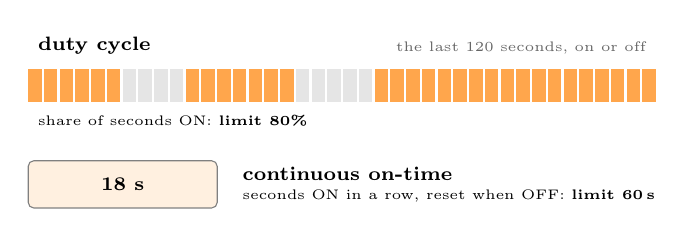
\begin{tikzpicture}[font=\scriptsize, >=stealth]
  % the duty-cycle window: the last 120 seconds, one cell per second (drawn as 40)
  \foreach \i in {0,...,39} {
    \pgfmathsetmacro{\on}{(\i<6 || (\i>=10 && \i<17) || \i>=22) ? 1 : 0}
    \ifdim\on pt=1pt
      \fill[orange!70] (\i*0.2, 0) rectangle ++(0.17, 0.42);
    \else
      \fill[black!10] (\i*0.2, 0) rectangle ++(0.17, 0.42);
    \fi
  }
  \node[anchor=south west, font=\scriptsize\bfseries] at (0, 0.48) {duty cycle};
  \node[anchor=south east, font=\tiny, text=black!60] at (7.97, 0.48)
    {the last 120 seconds, on or off};
  \node[anchor=north west, font=\tiny] at (0, -0.05) {share of seconds ON: {\bf limit 80\%}};

  % the continuous on-time counter
  \draw[rounded corners=2pt, draw=black!50, fill=orange!12] (0,-1.35) rectangle (2.4,-0.75);
  \node[font=\scriptsize\bfseries] at (1.2,-1.05) {18 s};
  \node[anchor=west, font=\scriptsize\bfseries] at (2.6,-0.92) {continuous on-time};
  \node[anchor=west, font=\tiny] at (2.6,-1.2) {seconds ON in a row, reset when OFF:
    {\bf limit 60\,s}};
\end{tikzpicture}\par}

\vspace{0.3cm}
Either limit exceeded: the heater goes to {\bf FAULT}.

\pause
\vspace{0.15cm}

\begin{block}{{\tt RESET\_STATISTICS}, an operator command}\small
Clears the duty-cycle buffer (the last 120 seconds) and sets the on-time counter to 0:
the record of how long the heater has been on is gone.
\end{block}

\end{frame}
%----------------------------------------
\begin{frame}[fragile]
  \frametitle{A proved theorem that was the wrong theorem} \small
\leanbadge{2}{bug found}{red!75!black}

\vspace{-0.3cm}
{\bf 1.}\ \ A violated safety limit leads to FAULT within one second (10 ticks):

\vspace{0.1cm}
\begin{lstlisting}[language=lean4]
theorem tick_sequence_corrects_safety (s) (params) :
  Reachable s params -> violatesSafetyLimits s params ->
  let ticks := List.replicate TICKS_PER_UPDATE SystemEvent.Tick
  (executeTrace params ticks s).currentState = HeaterState.FAULT
\end{lstlisting}

\vspace{-0.05cm}
{\bf Proved.} But the 10 events are {\em only} ticks: nothing else may happen.

\pause

\vspace{0.25cm}
\tikz[remember picture, overlay]{\node[anchor=east] at ([xshift=-0.35cm]current page.east |- 0,0.05) {\ideaicon[0.9]};}%
\parbox{0.86\textwidth}{{\bf 2.}\ \ Corrected: the heater reaches {\bf FAULT} for {\em any} events, as long as
10 of them are ticks.}

\vspace{0.1cm}
\begin{lstlisting}[language=lean4]
theorem safety_response_within_one_second (s) (params) (trace) :
  Reachable s params -> violatesSafetyLimits s params ->
  countTicks trace = TICKS_PER_UPDATE -> ReachesFault s params trace
\end{lstlisting}

\pause
\vspace{-0.05cm}
{\bf False.} {\tt RESET\_STATISTICS}, sent while the heater is ON, clears the safety
counters but leaves the heater on: repeated, FAULT never comes, and the heater stays on
{\bf forever}.

\end{frame}

%----------------------------------------
\begin{frame}[fragile]
  \frametitle{The fix, and the third theorem} \small
\leanbadge{2}{bug found}{red!75!black}

\vspace{-0.1cm}
{\bf 3.}\ \ Fixed in the C++: the reset is rejected while ON.

\vspace{0.1cm}
\begin{lstlisting}[style=cpp]
void HeaterActuator::RESET_STATISTICS_cmdHandler(...) {
    if (m_currentState == HeaterState::ON) { ... EXECUTION_ERROR; return; }
    ...                                // only now clear the counters
\end{lstlisting}

\pause
\vspace{0.15cm}

And the goal widened, from {\tt ReachesFault} to {\tt SafetyResolved}: FAULT, {\em or} the
violation gone.

\vspace{0.1cm}
\begin{lstlisting}[language=lean4]
theorem safety_response_within_one_second (s) (params) (trace) :
  Reachable s params -> violatesSafetyLimits s params ->
  countTicks trace = TICKS_PER_UPDATE -> SafetyResolved s params trace
\end{lstlisting}

\vspace{-0.05cm}
{\bf Proved.}

\end{frame}
%----------------------------------------
\begin{frame}[fragile]
  \frametitle{What does ``resolved'' mean?} \small
\leanbadge{2}{bug found}{red!75!black}

\vspace{-0.1cm}
The heater faults, {\em or} the violation is gone:

\begin{lstlisting}[language=lean4]
def SafetyResolved (s) (params) (trace) : Prop :=
  exists pre suf, trace = pre ++ suf /\
    ((executeTrace params pre s).currentState = HeaterState.FAULT \/
     not (violatesSafetyLimits (executeTrace params pre s) params))
\end{lstlisting}

\pause
\vspace{0.15cm}

``Gone'' is measured on the {\bf counters}: the duty-cycle buffer and the on-time.

\begin{itemize}\small
\item {\tt RESET\_STATISTICS} sets both to 0, so the violation is ``gone'', while the
      heater is still on.
\item So the definition cannot tell a heater turned OFF from {\bf wiped evidence}.
\end{itemize}

\pause
\vspace{0.15cm}

\begin{block}{The unfixed code satisfies this theorem too}\small
The property was corrected, then weakened again: it no longer excludes the bug. Only
the C++ fix does, by rejecting the reset while ON.
\end{block}

\end{frame}
%----------------------------------------
\begin{frame}[fragile]
  \frametitle{The whole system, composed along the topology} \small
\leanbadge{3}{proved}{green!45!black}

\vspace{-0.2cm}
\whereami{ctl,act}

\vspace{0.3cm}
\iconllm[0.85]\ A system model from {\tt topology.fpp}. The controller is modelled in
full; the actuator is {\bf abstracted} to OFF, ON or FAULT, and may fault at any time.

\vspace{0.3cm}
\begin{lstlisting}[language=lean4]
structure SystemState where
  sensor : Sensor.State
  averager : Averager.State
  controller : Controller.State
  actuator : Actuator.State
\end{lstlisting}

\vspace{0.25cm}
\begin{lstlisting}[language=lean4]
theorem system_step_fault_forces_manual_mode (sys) (p) (hi lo) :
  (systemStep sys p true hi lo).controller.controlMode = manual
\end{lstlisting}

\vspace{0.1cm}
{\small An actuator fault puts the controller in manual mode, from {\em any} state.}

\vspace{0.2cm}
{\scriptsize The Actuator abstraction was chosen by the LLM for convenience (no Mathlib): sound for the
controller's reaction to faults, but blind to what the actuator does after one as we shall see next.}

\end{frame}
         %  4 min   models, properties, proofs, the deployment
%----------------------------------------
\begin{frame}[fragile]
  \frametitle{Instrumenting the generated code for monitoring} \small
\dejavubadge{}{instrumentation}{black!55}

\vspace{-0.2cm}
\fprime{} generates a C++ class per port type. In a verification build, each one gets a
subclass that records the call, then forwards it:

\vspace{0.1cm}
\begin{lstlisting}[style=cpp]
class OutputHeaterCommandPort : public OutputHeaterCommandPortBase {
  public:
    void invoke(const TempControl::HeaterState& heaterState) const {
      Fcheck::record(getObjName(), heaterState);
      OutputHeaterCommandPortBase::invoke(heaterState);
    }
};
\end{lstlisting}

\pause
\vspace{0.25cm}
The raw record: time, port, event id, timestamp, severity, argument bytes:

\vspace{0.1cm}
\begin{lstlisting}[style=shell]
92281991262,heaterActuator_eventOut_OutputPort[0],536903680,
1792172611.792976,x06,x0000000200000001
\end{lstlisting}

\pause
\vspace{0.25cm}
translated with the \fprime{} dictionary into a named event:

\vspace{0.1cm}
\begin{lstlisting}[language=qtl]
heaterActuator_STATE_CHANGED("FAULT", "ON")
\end{lstlisting}

\end{frame}

%----------------------------------------
\begin{frame}[fragile]
  \frametitle{A temporal property, in \dejavumt{}} \small
\dejavubadge{4}{violated}{red!75!black}

\vspace{0.3cm}
Using the event {\tt STATE\_CHANGED} from the generated vocabulary (slide 7):

\vspace{0.3cm}
\begin{lstlisting}[language=qtl]
// The actuator never goes straight from FAULT to ON: FAULT goes through OFF.
prop fault_cleared_before_heating :
  !heaterActuator_STATE_CHANGED("FAULT", "ON")
\end{lstlisting}

\end{frame}

%----------------------------------------
\begin{frame}[fragile]
  \frametitle{The violation, on a recorded run} \small
\dejavubadge{4}{violated}{red!75!black}

Scenario: heat until the heater has been on too long, then turn it on by hand.

\begin{lstlisting}[style=shell]
70.870 s  heaterActuator_STATE_CHANGED(ON, FAULT)
70.870 s  faultNotify
71.281 s  heaterController_MODE_CHANGED(MANUAL)
77.846 s  cmd_heaterController_HEATER_MANUAL_CMD(ON)
77.846 s  heaterCmd(ON)
77.846 s  heaterActuator_STATE_CHANGED(FAULT, ON)    <- violated here
\end{lstlisting}

\pause

\begin{block}{A real hazard}\small
The controller, in manual mode, allows the operator's ON straight on from FAULT.
The heater now runs with its {\bf safety limits off}.
\end{block}

\pause

\begin{block}{The same kind of bug as {\tt RESET\_STATISTICS}}\small
An operator command gets around the fault protection. The fix for the first bug,
found with \lean{}, did not cover this path.
\end{block}

\end{frame}

%----------------------------------------
\begin{frame}[fragile]
  \frametitle{Why FAULT $\to$ ON is dangerous: the latches} \small
\dejavubadge{4}{consequence}{black!55}

\vspace{-0.35cm}
\whereami{act}

Each limit has a {\bf latch}: a flag that, once set, stays set. A set latch means
``this fault has already been reported'', so the check does not fire every second.

\begin{lstlisting}[style=cpp]
if (dutyCycle > maxDutyCycle && !m_dutyCycleFaultTriggered) {
    setFaultState();                      // the heater goes to FAULT
    m_dutyCycleFaultTriggered = true;     // reported: stay silent from now on
}
...
if (oldState == FAULT && newState == OFF) {
    m_dutyCycleFaultTriggered = false;    // only FAULT -> OFF re-arms it
    m_continuousOnTimeFaultTriggered = false;
}
\end{lstlisting}

\pause

\begin{block}{The expected flow: FAULT $\to$ OFF $\to$ ON}\small
Going through OFF clears the latches, so both limits are checked again once the heater
is back on.
\end{block}

\end{frame}
%----------------------------------------
\begin{frame}
  \frametitle{Four properties, three levels} \small

\vspace{-0.25cm}
\begin{center}\small
\renewcommand{\arraystretch}{1.2}
\begin{tabular}{|c|>{\raggedright\arraybackslash}p{2.3cm}|>{\raggedright\arraybackslash}p{3.2cm}|>{\raggedright\arraybackslash}p{4.0cm}|}
\hline
\rowcolor{blue!10}
 & {\bf checked on} & {\bf property} & {\bf holds?}\\
\hline
1 & \lean{}\newline controller model & a hot reading turns the heater off
  & {\color{red!70!black}\bf false} as stated;\newline {\color{green!45!black}\bf true} given the proved\newline invariant \mbox{\tt hysteresis > 0}\\
\hline
2 & \lean{}\newline actuator model & a violated limit leads to FAULT, whatever else happens
  & {\color{red!70!black}\bf false}: operator sends\newline {\tt RESET\_STATISTICS}\\
\hline
3 & \lean{}\newline system model & a fault puts the controller in manual mode
  & {\color{green!45!black}\bf true}\\
\hline
4 & \dejavumt{}\newline the real code & the heater never goes directly from FAULT to ON
  & {\color{red!70!black}\bf false}: operator sends\newline {\tt HEATER\_MANUAL\_CMD(ON)}\\
\hline
\end{tabular}
\end{center}

\vspace{0.05cm}
{\small 2 and 4: an operator command gets around the fault protection.}

\end{frame}
%----------------------------------------
\begin{frame}
  \frametitle{What each method covers} \small

\vspace{0.1cm}
{\centering
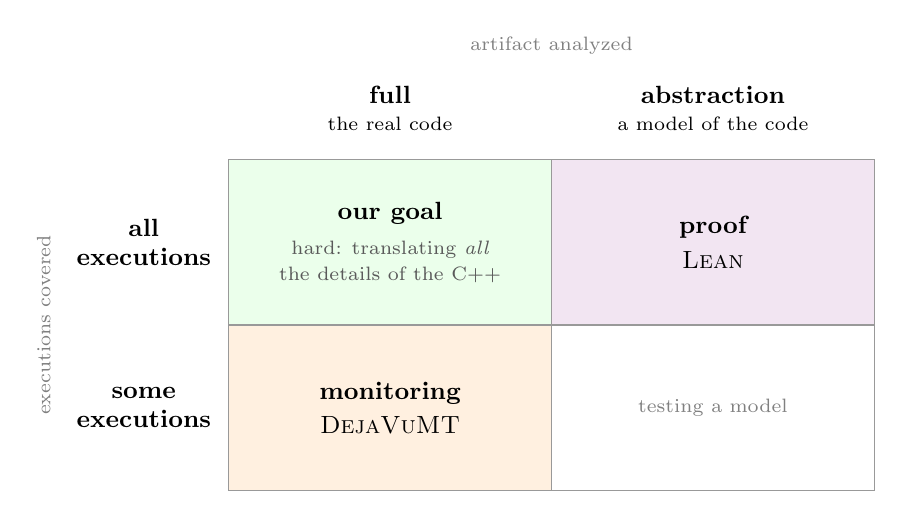
\begin{tikzpicture}[
  font=\small,
  cell/.style={draw=black!40, minimum width=4.1cm, minimum height=2.1cm, align=center},
  head/.style={font=\small\bfseries, align=center}
]
  % column heads: the artifact analyzed
  \node[head] at (2.05, 4.75) {full\\[-1pt]{\scriptsize\mdseries the real code}};
  \node[head] at (6.15, 4.75) {abstraction\\[-1pt]{\scriptsize\mdseries a model of the code}};
  \node[font=\scriptsize, gray] at (4.1, 5.55) {artifact analyzed};

  % row heads: the executions covered
  \node[head, anchor=east] at (-0.1, 3.05) {all\\executions};
  \node[head, anchor=east] at (-0.1, 0.95) {some\\executions};
  \node[font=\scriptsize, gray, rotate=90] at (-2.35, 2.0) {executions covered};

  \node[cell, fill=green!8] (fa) at (2.05, 3.05) {{\bf our goal}\\[2pt]{\scriptsize\color{black!65}hard: translating {\em all}}\\[-1pt]{\scriptsize\color{black!65}the details of the C++}};
  \node[cell, fill=violet!10] (pa) at (6.15, 3.05) {{\bf proof}\\[2pt]\lean{}};
  \node[cell, fill=orange!12] (fs) at (2.05, 0.95) {{\bf monitoring}\\[2pt]\dejavumt{}};
  \node[cell] (ps) at (6.15, 0.95) {{\color{gray}\scriptsize testing a model}};
\end{tikzpicture}\par}

\end{frame}
      %  4 min   instrumentation and DejaVuMT
%----------------------------------------
\begin{frame}
  \frametitle{Conclusion} \small

\begin{enumerate}\small

      \item LEAN proofs went through automatically, which is a game changer - so far.

      \pause

      \item But writing the specification is still hard:
      \begin{itemize}\small
      \item which properties to write; One has to know what the ``knobs'' are and how to turn them.
      \item getting a single property right. The {\tt RESET\_STATISTICS} bug hid behind a
            proved but too weak property.
      \end{itemize}

      \pause

      \item Properties are associated with natural language explanations.

      \pause

      \item Is the model the code? The FAULT $\to$ ON bug hid behind a proved but too weak
      model. Tricky problems include memory safety, aliasing, and concurrency.

      \pause

      \item One can also use the LLM to find problems in the code and generate a model, 
            e.g. in Promela (Spin) to demonstrate it.
      
      \pause

      \item An LLM can perform static analysis, checking against coding standards.

      \pause

      \item One can of write the spec first, then the code, and then prove the code against the spec.

\end{enumerate}

\end{frame}
      %  3 min   automation bias, challenges
%----------------------------------------
\begin{frame}

\vfill
\centering {\Large\bf Questions?}

\vfill

\end{frame}
    %  --

\end{document}
